
\documentclass[AMA,STIX1COL]{WileyNJD-v2}
\usepackage{moreverb}
%\usepackage{amsmath}
\usepackage{tikz}
\usepackage{mathtools}
\mathtoolsset{showonlyrefs}
\usetikzlibrary{patterns} 
\usetikzlibrary{shapes}
\usetikzlibrary{snakes}
\usetikzlibrary{pgfplots.groupplots}
\usetikzlibrary{external} % avoid the systematic compilation of figures
\usetikzlibrary{spy,backgrounds}
\usetikzlibrary{decorations.markings}
\usetikzlibrary{arrows.meta}
\RequirePackage{amsmath,eucal,stmaryrd,mathrsfs}

\usepackage{pgfplotstable}

%%%%
% Define user commands 
\newcolumntype{M}[1]{>{\centering\arraybackslash}m{#1}}
\newcolumntype{N}{@{}m{0pt}@{}}

\newcommand{\vect}[1]{{\mathbf{\boldsymbol{#1}}}}
\newcommand{\Ac}{\mathcal{A}}
\newcommand{\Bc}{\mathcal{B}}
\newcommand{\Vc}{\mathcal{V}}
\newcommand{\Vscr}{\mathscr{V}}
\newcommand{\Pscr}{\mathscr{P}}
\newcommand{\Rbb}{\mathbb{R}}

\newcommand{\nablav}{\vect{\nabla}}
\newcommand{\divv}{\nablav \cdot \,}
\newcommand{\abs}[1]{\left\vert#1\right\vert}

\newcommand{\drond}[2]{\frac{\partial #1}{\partial #2}}

\renewcommand{\(}{\left(}
\renewcommand{\)}{\right)}
\renewcommand{\[}{\left[}
\renewcommand{\]}{\right]}

\newcommand{\bra}[1]{\left[#1\right]}
\newcommand{\mat}[1]{\begin{matrix}#1\end{matrix}} 
% Matrice avec crochets
\newcommand{\matrice}[1]{\bra{\mat{#1}}}

\definecolor{Purple}{RGB}{120,28,129}
\definecolor{Orange}{RGB}{231,133,50}
\definecolor{Blue}{RGB}{63,96,174}
\definecolor{Red}{RGB}{217,33,32}
\definecolor{Duck}{RGB}{83,158,182}
\definecolor{Green}{RGB}{109,179,136}
\definecolor{Yellow}{RGB}{202,184,67}
%%%% 

\newcommand{\review}[1]{\color{Blue}#1\color{black}}
\newcommand{\note}[1]{\color{Red}#1\color{black}}

\renewcommand{\thefootnote}{\fnsymbol{footnote}}

\articletype{Article Type}%

\received{}
\revised{}
\accepted{}
        
\raggedbottom

\begin{document}

\title{Stability properties of the Discontinuous Galerkin Material Point Method for hyperbolic problems in one and two space dimensions}

\author[1]{Adrien Renaud*}
\author[1]{Thomas Heuz{\'e}}
\author[1]{Laurent Stainier}

\authormark{\textsc{Renaud et al}}


\address[1]{\orgdiv{Research Institute in Civil and Mechanical Engineering}, \orgname{Ecole Centrale de Nantes}, \orgaddress{\country{France}}}
% \address[2]{\orgdiv{Org Division}, \orgname{Org Name}, \orgaddress{\state{State name}, \country{Country name}}}
% \address[3]{\orgdiv{Org Division}, \orgname{Org Name}, \orgaddress{\state{State name}, \country{Country name}}}

\corres{Adrien Renaud \email{adrien.renaud@ec-nantes.fr}}

\presentaddress{Research Institute in Civil and Mechanical Engineering (GeM, UMR 6183 CNRS)\\
	Ecole Centrale de Nantes \\
	1 rue de la No\"e, Nantes}

      \abstract[Summary]{
        In this paper, stability conditions are derived for the Discontinuous Galerkin Material Point Method \cite{DGMPM,Thesis} on the scalar linear advection equation for the sake of simplicity and without loss of generality.
        %The corresponding discrete system that is derived is based on either the forward Euler or the second-order Runge-Kutta (RK2) time discretizations, and on the computation of numerical fluxes at cell faces by means of the Donor-Cell Upwind (DCU) \cite{Leveque} or the Corner Transport Upwind (CTU) \cite{Colella_CTU} methods for multi-dimensional problems.
        The corresponding discrete system is based on the computation of numerical fluxes at cell faces by means of the Donor-Cell Upwind (DCU) \cite{Leveque} or the Corner Transport Upwind (CTU) \cite{Colella_CTU} methods for multi-dimensional problems.
        \review{The scheme equation of the DGMPM applied to the scalar linear advection equation is derived, combined with RK2 for one-dimensional cases, and with the forward Euler algorithm for two-dimensional problems.
        These equations are based on the assumption that all cells of a Cartesian background grid contain at least one particle and can be easily extended to regular grids, that is, rectangle rather than square elements. }
        The von Neumann linear stability analysis then enables the writing of mathematical expressions depending on the Courant number and the distribution of particles in the DGMPM arbitrary grid which, in turn, allow to compute the critical Courant number for a given space discretization.
        \review{As already highlighted \cite{DGMPM}, the DGMPM is equivalent to the first-order finite volume method if one particle lies in each element of the computational grid.
          Hence, the Courant number can be set to unity in that case.
          However, increasing the number of material points in the cells may lead to a decrease in the critical Courant number depending on the time discretization considered and the position of the particles.
          The study of particular configurations including symmetrical or asymmetrical distributions of material points with respect to the element centers is then proposed. 
        }
      }

\keywords{Discontinuous Galerkin Material Point Method, Stability analysis, Critical CFL number, Hyperbolic problems, Corner Transport Upwind method}

\maketitle

\section{Introduction}
\label{sec:introduction}
The numerical simulation of physical problems modeled by means of hyperbolic partial differential equations involves the solution of possibly discontinuous waves.
%
The precise tracking of those waves is of major importance in solid mechanics, especially for history-dependent constitutive equations, as it allows to properly assess the residual states.
\review{More specifically, high-speed forming techniques such that electromagnetic forming \cite{Formage} also requires the tracking of solid interfaces.}   
% \note{(a) Examples of applications that involve large deformations}
% \note{Discontinuities + Large deformations!!}
%
Nevertheless, the accurate simulation of such problems can be prevented by several reasons.
%% Mesh-based Lagrangian
First, Lagrangian formulations of mesh-based approaches such as the widely used Finite Element (FEM) \cite{Belytschko} and Finite Volume (FVM) \cite{Leveque} methods become less accurate for very large deformations due to sever distortions of the mesh.
%% Mesh-based Eulerian and ALE
Although those instabilities can be avoided by resorting to Eulerian or Arbitrary Lagrangian-Eulerian formulations, other difficulties arise owing to additional diffusive projections of fields.
%% Time integration
Second, it is well-known that explicit finite element schemes can exhibit numerical noise near sharp solutions that can be hard to remove with artificial viscosity without loss of accuracy.
Such oscillations can nevertheless be removed from FVM solutions due to numerical fluxes involved in the formulation, allowing the building of Total Variation Diminishing (TVD) schemes \cite{Harten}.
%% DG
The Discontinuous Galerkin approximation in space \cite{NeutronDG}, combined with FEM (DGFEM), enables to take advantage of similar interface fluxes so as to construct Total Variation Diminishing in the Means (TVDM) finite element procedures \cite{Cockburn}.
%% Time integration in DGFEM -> STDG
While the introduction of the DG approximation within FEM schemes enables to avoid non-physical oscillations, providing the use of suitable limiters \cite{vanLeer_Limiters}, these approaches are constrained by a restrictive CFL condition \cite{DGFEM_CFL} and hence, suffer from numerical diffusion.
Space-time DGFEM formulations \cite{ST_DGFEM1} enable to circumvent this drawback but are nonetheless subject to mesh entanglement.
%\review{Moreover, the satisfaction of the compatibility condition between reference and updated configurations, through the Piola identity, is not a straightforward undertaking in Lagrangian formulations \cite{Vilar_PiolaIdentity,LagrangianDG_thesis}, which is also the case for finite volumes \cite{Haider_FVM}.
%In other words, updating the geometry based on discontinuous velocities and deformation gradients across element faces may lead to discontinuities in the displacement vector.}


%% MPM
One possibility to avoid mesh tangling instabilities while providing a material description of the motion is to use mesh-free approaches such as those of the Particle-In-Cell (PIC) family \cite{PIC} and, in particular, the Material Point Method \cite{Sulsky94}.
The MPM is based on a dual discretization of a domain made of a collection of material points lying in an arbitrary grid.
A discrete system is solved on the grid, whereas the loading history is stored at particles during the motion so that field projections, which introduce some freedom into the scheme, are required.
%
Indeed, the updated velocity at the grid level can be directly interpolated to the particles according to the original PIC procedure.
Alternatively, the particle velocities can be updated by interpolating the nodal acceleration resulting from the solution of the discrete system, as introduced in PIC by the FLuid Implicit Particle method (FLIP) \cite{FLIP}.
The latter allows to reduce numerical diffusion at the cost of spurious oscillations \cite{PIC_Nishiguchi}.
Recently, a tunable mapping procedure, based on a parameter $m$ that completely eliminates the noise in MPM solutions, has been proposed in the Extended PIC of order $m$ (XPIC(m)) \cite{XPIC}.
A classical interpolation is selected for $m=1$ whereas the mapping tends to FLIP one as $m\rightarrow \infty$.
Nevertheless, the numerical diffusion still prevents from capturing (discontinuous) waves.

%% DGMPM 
\review{
  %A different point of view, which is followed in the Discontinuous Galerkin Material Point Method (DGMPM) \cite{DGMPM,Thesis}, is that the numerical diffusion exhibited by the PIC can be limited by reducing the domain of influence of nodes rather than modifying the projections themselves.
  Note also that the numerical diffusion exhibited by the PIC can be limited by reducing the domain of influence of nodes rather than modifying the projections themselves.
  This approach is followed in the Discontinuous Galerkin Material Point Method (DGMPM) \cite{DGMPM,Thesis}.
  The introduction of the DG approximation within the MPM, combined with the use of the PIC projection, thus aims at providing non-oscillating discontinuous solutions with low numerical diffusion due to the support of the shape functions that reduces to one cell.
  Therefore, the DGMPM enables to take advantage of space-DGFEM and MPM in order to accurately follow waves in finite-deforming media.
}
%
In that method, the weak form of a system of conservation laws is written on an arbitrary grid and numerical fluxes arising from the DG approximation are computed at cell faces by means of an approximate Riemann solver.
Those intercell fluxes allow to take into account the characteristic structure of hyperbolic problems, and in particular the transverse propagation of waves through the use of the Corner Transport Upwind method (CTU) \cite{Colella_CTU} developed for finite volumes.
The CTU is however reformulated in order to fit the DGMPM approximation, in which fields are edge-wise constant in Riemann problems rather than cell-wise constant as it is the case for FVM.
%% Arbitrary grid
Furthermore, as in MPM, all the fields are stored at material points moving in the arbitrary grid, the mapping between nodes and particles being made with PIC projection so that non-oscillating solutions are provided.
\review{Hence, the geometry is updated at the particles level based on a single-valued velocity field. %, in such a way that the difficulties related to the Piola identity are expected to vanish, though it has not been shown so far.
  %% Total Lagrangian
  As a first development step, the DGMPM has been constructed upon a total Lagrangian formulation.
  %
  The numerical results provided by the method for a plane wave problem in a finite-deforming hyperelastic material showed excellent agreement with the exact solution consisting of either a shock or a rarefaction wave \cite{DGMPM}.
  It is worth noticing that similar results can be obtained with the FVM written in the reference configuration, the key point being however that the update of the geometry is straightforward in the DGMPM.
  %
  Furthermore, an interesting feature of the method consists in allowing the employment of mesh adaption strategies so that waves can be accurately captured in the current configuration.
  On the other hand, only linear shape functions leading to a first-order accuracy \cite{Thesis} have been considered, the extension of the method to higher-order approximations being the object of ongoing works.
  The low-order approximation is however not seen as a shortcoming for now since the development of the method has been focused so far on capturing discontinuous solutions for which the accuracy of any numerical scheme falls to one \cite{Leveque}.
}
%Although the equations of solid mechanics are solved in the reference configuration according to a total Lagrangian formulation, an interesting feature of the method consists in allowing the employment of mesh adaption strategies so that waves can be accurately captured in the current configuration.
%% CFL depending on the space discretization
Nonetheless, the stability of the DGMPM highly depends on the distribution of particles inside the computational grid.
Indeed, the stability analysis of the one-dimensional DGMPM scheme coupled to the forward Euler time integration \cite{DGMPM} yields a stability condition that depends on the space discretization and the CFL number.
%
Conversely, one can ensure the stability for a given distribution of material points by finding the CFL number satisfying the aforementioned relation.
%
Such a condition, which does not exist for the MPM and other DGMPM discretizations, is crucial since it allows to: (i) ensure the stability of the scheme while minimizing the numerical diffusion; (ii) adapt the Courant number when the grid is reconstructed; (iii) adapt the grid so that a given CFL condition is satisfied.
It is the purpose of this paper to provide the stability conditions for the one-dimensional DGMPM scheme combined with the two-stage second-order Runge-Kutta (RK2) time discretization and for the two-dimensional DGMPM coupled to the forward Euler algorithm.
\review{
  Although the solution of linear equations is considered here, the results presented must be put into the context of the problems aimed by the method, involving large deformation, and for which the DGMPM enables plenty of perspectives. 
  }

%% Organization of the paper
In the following, the DGMPM discrete system for the multi-dimensional scalar linear advection equation is derived and the computation of interface fluxes, as well as the solution scheme, are recalled in section \ref{sec:dgmpm}.
In particular, we shall see that the adaptation of the Corner Transport Upwind method (CTU) \cite{Colella_CTU} to DGMPM leads to the same corrections of intercell fluxes as for finite volumes.
Second, the system resulting from the combination of DGMPM and RK2 discretization is specialized to one-dimensional problems in section \ref{sec:1d_stab} so that the von Neumann linear stability analysis is carried out.
At last, the same approach is followed in section \ref{sec:2d_stab} for the DGMPM scheme coupled to the forward Euler time integration applied to the two-dimensional problem.


%%% Local Variables:
%%% mode: latex
%%% TeX-master: "manuscript"
%%% End:


\section{Discrete system for the scalar linear advection equation}
\label{sec:dgmpm}
Consider a solid domain with %constant mass density $\rho$ and
constant volume $\Omega \in \Rbb^3$, bounded by the surface $\partial \Omega$ within the time interval $t \in \tau=[0,T]$.
% Although the DGMPM has been developed within the finite strain framework, the equations considered here involve a configuration $\Omega$ that does not change during the deformation.
In that domain, a material particle is located in the Cartesian coordinates system by the vector $\vect{x}=x_\alpha \vect{e}_\alpha$, following the convention of implicit summation over repeated indices.

\subsection{The model equation}
We focus here on the transport of an arbitrary scalar quantity $q$ in that domain, governed by the advection equation:
\begin{equation}
  \label{eq:advection_equation}
  \drond{q}{t}(\vect{x},t) +  \nablav \cdot \vect{F}(\vect{x},t) = 0 \quad \forall \:\vect{x},t \in \Omega \times \tau
\end{equation}
where $\nablav \cdot (\bullet)$ is the right divergence operator, and $\vect{F}=q(\vect{x},t)s_\alpha \vect{e}_\alpha$, the flux vector.
In the expression of the flux vector, $s_\alpha \in \Rbb$ is the speed at which the quantity $q$ is advected in direction $\vect{e}_\alpha$.
For the linear advection equation considered here, these celerities are constant and equation \eqref{eq:advection_equation} can be rewritten as:
\begin{equation}
  \label{eq:advection_equation_sum}
  \drond{q}{t}(\vect{x},t) +  s_\alpha \drond{q}{x_\alpha}(\vect{x},t) = 0\quad \forall \:\vect{x},t \in \Omega \times \tau
\end{equation}

\subsection{DGMPM space discretization}
The continuum body $\Omega$ is discretized into a set of $N_p$ material points in a Cartesian grid made of $N_n$ nodes and $E$ non-overlapping cells of volume $\Omega^e$.
The boundary of the computational domain is defined by the set of faces separating empty cells from those containing particles (see figure \ref{fig:domain} for a two-dimensional example).
\begin{figure}[ht]
  \centering
  \begin{tikzpicture}[scale=0.8]
  % \draw[step=1.0,black,thin] (-3.,-1.) grid (3,4.);
  \draw[white] (-3,-1) -- (3,-1) -- (3,4) -- (-3,4) -- (-3,-1);
  \begin{scope}[scale=0.5]
    \draw[thick] (-3,0.6) .. controls +(1,0) and +(-1,0) .. (0,1.8)  
    .. controls +(1,0) and +(0,-3) .. (5,3.2) 
    .. controls +(0,2) and +(2,0)  .. (0,5.2) 
    .. controls +(-1,0) and +(0,3) .. (-4.5,2.2) 
    .. controls +(0,-1) and +(-1,0).. (-3,0.6) ;
    \begin{scope}  % pour limiter la portée du clip
      \clip (-3,0.6) .. controls +(1,0) and +(-1,0) .. (0,1.8) 
      .. controls +(1,0) and +(0,-3) .. (5,3.2)
      .. controls +(0,2) and +(2,0)  .. (0,5.2)
      .. controls +(-1,0) and +(0,3) .. (-4.5,2.2)
      .. controls +(0,-1) and +(-1,0).. (-3,0.6);
    \end{scope}
    \node[below] at (0,1) {$\Omega_t$};
  \end{scope}
  \draw [->,very thick,gray] (3.,1.5) -- (3.6,1.5);
\end{tikzpicture}
  \caption{Representation of a continuum body by a set of material points in a regular grid in $\Rbb^2$.}
  \label{fig:domain}	
\end{figure}
%%%%%
Even though MPM, and in turn DGMPM, have been developed for solid dynamics based on the balance equation of linear momentum, the formulation can be extended to equation \eqref{eq:advection_equation} by means of a fictitious mass density $\rho$.
Indeed, the methods rely on the representation of the mass density that weights the time partial derivative of the hyperbolic equation by means of a delta Dirac characteristic function:
%%%%
%MPM and DGMPM formulations for solid dynamics are based on representation of the mass density arising in the linear momentum balance equation by means of a delta Dirac characteristic function.
%%%%
% In that computational grid, the mass density is described based on the delta Dirac characteristic function and particles masses:
\begin{equation}
  \label{eq:mass_density_DGMPM}
  \rho\(\vect{x}\) =  \sum_{I=1}^{N_p} m_I \delta\(\vect{x}^I - \vect{x}\)
\end{equation}
where $\vect{x}^I$ is the position of the $I$th material point and $m_I$ the associated mass.
In the following, a unit mass density is assumed to derive the DGMPM.
% Even though equations \eqref{eq:advection_equation} and \eqref{eq:advection_equation_sum} do not involve the mass density, the approximation \eqref{eq:mass_density_DGMPM} is used hereinafter with a unit mass density.
Analogously to FEM and MPM, the quantity $q$ is approximated on the background grid as:
\begin{equation}
  \label{eq:DGMPM_node2points}
  q(\vect{x},t) = \sum^{N_n}_{i=1} S_{i}(\vect{x})q^i(t) 
\end{equation}
with $q^i$ the quantity at node $i$ and $S_{i}(\vect{x})$ the shape function attached to that node.
Note that the convention of denoting particle and nodal fields by uppercase and lowercase indices respectively is used in the remainder of the paper.

The key idea of DG methods is to allow jump of fields across mesh elements faces by using broken polynomial spaces for the approximate solution \cite{DiPietro}:
\begin{equation}
\Vscr^k = \{ \Vc \in H^k(\Omega^e) \} \quad ;\quad \Vscr_h^k = \{\Vc \in \Pscr^k(\Omega^e) \} \subset \Vscr^k
\end{equation}
$H^k(\Omega^e)$ being the Sobolev space, and $\Pscr^k(\Omega^e)$ the space of polynomials of degree $k$ in $\Omega^e$.
We restrict our attention here to linear polynomials ($k=1$).
Multiplying equation \eqref{eq:advection_equation} by a test function $\Vc$ yields the element-wise weak formulation of the problem:
\begin{equation}
  \label{eq:weak_form}
  \begin{aligned}
    &\textit{Find $q \in \Vscr_h^1$ such that }\forall e \\
    &\int_{\Omega^e} \Vc \drond{q}{t} \: d\Omega + \int_{\Omega^e}  \Vc \:  \nablav \cdot \vect{F}  \: d\Omega    = 0 \quad \forall \: \Vc,t \in  \Vscr_h^1\times \tau
  \end{aligned}
\end{equation}
Then, the use of Gauss' divergence theorem leads to:
\begin{equation}
  \label{eq:DGMPM_weak_form}
  \begin{aligned}
    &\textit{Find $q \in \Vscr_h^1$ such that }\forall e \\
    &\int_{\Omega^e} \[\drond{q}{t} \Vc - \vect{F} \cdot \nablav \Vc \] d\Omega   + \int_{\partial \Omega^e} \(\vect{F}\cdot \vect{n}\)  \Vc \: d\Gamma = 0 \quad \forall \: \Vc,t \in  \Vscr_h^1\times \tau
  \end{aligned}
\end{equation}
where $\partial \Omega^e$ is the boundary of the $e$th element with outward normal vector $\vect{n}$, and $\nablav(\bullet)$ is the gradient operator.
%The dot operator $\Fcb\cdot \vect{N}$ denotes the inner product between the outward normal vector and every component of the flux, thus yielding the intercell flux, written $\Fcb_N$ for simplicity.
The inner product $\vect{F}\cdot \vect{n}$, corresponding to intercell flux, is written $F_n$ for simplicity.
Next, the introduction of specific fields:
\begin{equation}
  \label{eq:specific_quantities}
  q = \rho \bar{q} \quad ; \quad \vect{F} = \rho \bar{\vect{F}} =\rho \vect{s} \bar{q}
\end{equation}
combined with the definition of mass density \eqref{eq:mass_density_DGMPM}, leads to the following weak form:
\begin{equation} 
  \label{eq:DGMPM_discrete_weak}
  \sum_{I=1}^{N_p} m_I\[\drond{\bar{q}}{t}  \Vc - \vect{s}\bar{q} \cdot \nablav \Vc \]_{|\vect{x}=\vect{x}^I} + \int_{\partial \Omega^e} F_n  \Vc \: d\Gamma = 0 \quad \forall \: \Vc,t \in  \Vscr_h^1\times \tau
\end{equation}
Introduction of the DGMPM approximation \eqref{eq:DGMPM_node2points} and arbitrariness of the test field in the weak form \eqref{eq:DGMPM_discrete_weak} finally provide the semi-discrete system that must be solved on the grid:
\begin{equation}
  \label{eq:DGMPM_semi_discrete}
  \sum_{I=1}^{N_p}\[ S_{iI} m_I S_{jI} \drond{\bar{q}^j}{t}  - \drond{S_{iI}}{x_\alpha} m_I S_{jI} s_\alpha \bar{q}^j\] + \int_{\Gamma_e} S_i(\vect{x}) F_n  \: d\Gamma =  0  \quad \forall \: t \in  \tau
\end{equation}
or, in matrix form:
\begin{equation}
  \label{eq:DGMPM_semi_discrete_matrix}
  M_{ij} \drond{\bar{q}^j}{t} - K^\alpha_{ij} s_\alpha \bar{q}^j + \hat{F}^i = 0  
\end{equation}
%The particles play the role of integration points in volume integrals owing to the delta Dirac characteristic function.
%Hence, as for MPM, the consistent mass matrix $M_{ij}$ may be singular due to reduced integration, so that the diagonally lumped mass matrix $M^L_i=\sum_{j=1}^{N_n} M_{ij}$ is used \cite{Love}.
\review{
  \begin{remark}
    As for MPM, the particle-based quadrature rule yields a consistent mass matrix $M_{ij}$ that may be singular due to reduced integration.
    This can be circumvented by resorting to the diagonally lumped mass matrix $M^L_i=\sum_{j=1}^{N_n} M_{ij}$ is used \cite{Love}.
    The aforementioned numerical trick, which is also employed in explicit FEM \cite{Belytschko} for efficiency purposes, can be avoided within the MPM owing to recent works.
    Indeed, the use of \textit{moving least squares} \cite{IMPM} or \textit{spline interpolation} \cite{MPM_BSpline1,MPM_BSpline2} techniques enables the evaluation of a reconstructed function ot Gauss point locations. 
    In these versions of the MPM, the particles are no longer seen as integration points. %so that higher-order approximations are possible regardless of the distribution of material points.
    Similar reconstructions can be considered within the DGMPM, which would amount to provide an arbitrary background grid to a DG scheme.
    This is, however, out of the scope of the present work.
  \end{remark}
  \begin{remark}
    The DGMPM discretization can be constructed upon regular grids that allow the straightforward building of an orthonormal approximation basis.
    In that case, the mass matrix is naturally diagonal provided the derivation of a modal formulation as can be done for DGFEM \cite{Hesthaven}.  
  \end{remark}
}

The DGMPM discrete system is finally derived by dividing the time interval $\tau$ into $N_t$ subintervals and using the explicit forward Euler method:
\begin{equation}
  \label{eq:DGMPM_discrete}
  M^L_i \frac{\bar{q}^{i,k+1} - \bar{q}^{i,k}}{\Delta t^{k} } = K^\alpha_{ij} s_\alpha\bar{q}^{j,k} - \hat{F}^{i,k}  
\end{equation}
where the superscripts $(\bullet)^{i,k}$ denote a field evaluated at node $i$ and time step $k$.
Alternatively, a second-order Runge-Kutta (RK2) explicit time discretization may be employed, leading to the following two-stage discrete form:
\begin{equation}
  \label{eq:DGMPM_discrete_RK2}
  \begin{aligned}
    & M^L_i \frac{\bar{q}^{i,k+1/2} - \bar{q}^{i,k}}{\Delta t^{k} } = \frac{1}{2}\(K^\alpha_{ij} s_\alpha\bar{q}^{j,k} - \hat{F}^{i,k}\)  \\
    & M^L_i \frac{\bar{q}^{i,k+1} - \bar{q}^{i,k}}{\Delta t^{k} } = K^\alpha_{ij} s_{\alpha}\bar{q}^{j,k+1/2} - \hat{F}^{i,k+1/2}
  \end{aligned}
\end{equation}

\subsection{Computation of intercell fluxes}
The relaxation of the continuity of fields across cells interfaces introduced by the DG approximation allows to define Riemann problems at element faces in the direction $x_n=\vect{x}\cdot{n}$:
\begin{equation}
  \label{eq:RP_mesh}
  \begin{aligned}
    &\drond{q}{t} + \drond{F_n}{x_n} = 0  \\
    & q(x_n,0)= \left\lbrace 
      \begin{aligned}
        & q^{-} \text{ if } x_n <0 \\
        & q^{+} \text{ if } x_n > 0
      \end{aligned}
        \right.
  \end{aligned}
\end{equation}
where the $q^{\pm}$ are downwind and upwind states.
The use of DG approximation can be seen as a duplication of nodes so that those states can be obtained by averaging nodal fields on each side of the interface as depicted in figure \ref{fig:2D_edge} for a two-dimensional case.
By doing so, only one Riemann problem per interface rather than nodal ones is considered, thus avoiding a dramatic increase in computational time.
%\review{Nevertheless, nodal Riemann problems might be considered for an extension of the method to higher-order approximations.}
\begin{figure}[h!]
  \centering
  \begin{tikzpicture}[scale=0.5]
  \draw (10.,0.) -- (12.,6.) ;
  \draw[fill=white] (9.85,0.1) circle (0.1) node [left] {$1$};	
  \draw[fill=white] (10.2,-0.0) circle (0.1) node [right] {$2$};	
  \draw[fill=white] (11.85,6.1) circle (0.1) node [left] {$4$};	
  \draw[fill=white] (12.2,6) circle (0.1) node [right] {$3$};	
  \draw[black] (9.85,0.1) circle (0.1) node [left] {$1$};	
  \draw[black] (10.2,-0.0) circle (0.1) node [right] {$2$};	
  \draw[black] (11.85,6.1) circle (0.1) node [left] {$4$};	
  \draw[black] (12.2,6) circle (0.1) node [right] {$3$};	
  \draw[->,very thick] (11.,3.) -- (12,3 -1/3) node [right,below] {$X_N$}; 
  \node at (8,3.5) {$\Ucb_{X_N^-} = \frac{\Ucb_1 + \Ucb_4}{2}$}; \node at (14.5,3.5) {$\Ucb_{X_N^+} = \frac{\Ucb_2 + \Ucb_3}{2}$};
\end{tikzpicture}

%%% Local Variables:
%%% mode: latex
%%% TeX-master: "../manuscript"
%%% End:

  \caption{Duplication of nodes at an interface and building of initial conditions of the Riemann problem (2D).}
  \label{fig:2D_edge}
\end{figure}
As for the original formulation of the DGMPM \cite{DGMPM}, the numerical flux at a given interface is based on the stationary solution $q^*$ of the Riemann problem \eqref{eq:RP_mesh} according to Godunov's method \cite{Godunov_method}.
For the linear advection, the stationary solution is simply that of the upwind side, namely:
\begin{equation}
  \label{eq:stationary_state}
  \left\lbrace
    \begin{aligned}
      & q^* = q^{-} \quad \text{if $s_n>0$}\\
      & q^* = q^{+} \quad \text{if $s_n<0$}
    \end{aligned}
    \right.
\end{equation}
where $s_n=\vect{s}\cdot\vect{n}$, so that the intercell flux at a given interface reads $F_n=s_n q^*$.

% \subsubsection{Transverse corrections}
The method derived above for the computation of normal fluxes can be seen as the Donor-Cell Upwind method (DCU) \cite{Leveque} in which only the influence of upwind neighbor cells is considered.
For multi-dimensional problems, however, waves can travel in several directions so that contributions coming from corner cells must be taken into account in order to improve accuracy and stability of the numerical scheme.
The Corner Transport Upwind method (CTU) \cite{Colella_CTU} consists in considering contributions propagating in bias and coming from upwind cells sharing only a node (in two dimensions) with another.
This approach has been developed for finite volumes in which fields are cell-wise constant and allows to improve the Courant condition.
The approach is now reformulated for DGMPM, based on edge-wise constant fields within Riemann problems.

At each cell interface, one defines left-going and right-going fluctuations as:
\begin{equation}
  \label{eq:fluctuations}
  \Ac^-(\Delta q) = F_n(q^*) - F_n(q^-) \quad ;  \quad \Ac^+(\Delta q) = F_n(q^+)-F_n(q^*) 
\end{equation}
From equation \eqref{eq:fluctuations} and the definition of the stationary state $q^*$ \eqref{eq:stationary_state}, one of the fluctuation obviously vanishes for the scalar linear advection equation.
The non-zero fluctuation, on the other hand, characterizes a wave that carries a jump discontinuity $\Delta q$ at speed $s_n$ in the direction $\vect{n}$.
This jump influences the state vector $q$ in the neighbor cell so that the the initial data in the Riemann problems formulated on adjacent edges are changed.
To illustrate the above discussion, let's consider the patch of two-dimensional regular grid cells of length $\Delta x$ shown in figure \ref{fig:ctu_perso}.
\begin{figure}[ht]
  \centering
  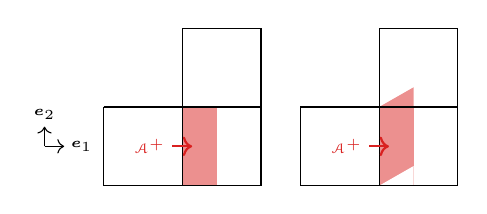
\begin{tikzpicture}[scale=0.5]
  \fill[Red!50] (0,0) rectangle (.875,-2);
  \draw (-2,0) -- (2,0.);\draw (0.,2) -- (0,-2.);\draw (0,2) -- (2,2);
  \draw (-2.,-2.) -- (2.,-2.);\draw (2,2.) -- (2,-2.);\draw (-2,-2) -- (-2,0);
  \begin{tiny}
    \draw[->,thick,Red] (-.25,-1.) node [left] {$\Ac^+$} -- (.25,-1.) ;
    \draw[->] (-3.5,-1.) -- (-3,-1.) node[right] {$\vect{e}_1$};
    \draw[->] (-3.5,-1.) -- (-3.5,-0.5) node[above] {$\vect{e}_2$};
  \end{tiny}
  \begin{scope}[shift={(5.,0.)}]
    \fill[Red!50] (0,0) rectangle (.875,-2);
    \fill[Red!50] (0,0) -- (.875,0) -- (.875,.5) -- (0.,0.); %% Red triangle
    \fill[white] (0,0-2) -- (.875,0-2) -- (.875,.5-2) -- (0.,0.-2); %% White triangle
    \draw (-2,0) -- (2,0.);\draw (0.,2) -- (0,-2.);\draw (0,2) -- (2,2);
    \draw (-2.,-2.) -- (2.,-2.);\draw (2,2.) -- (2,-2.);\draw (-2,-2) -- (-2,0);
    \begin{tiny}
      \draw[->,thick,Red] (-.25,-1.) node [left] {$\Ac^+$} -- (.25,-1.) ;
    \end{tiny} 
  \end{scope}
\end{tikzpicture}

%%% Local Variables:
%%% mode: latex
%%% TeX-master: "../../presentation"
%%% End:

  \caption{Illustration of the influence of fluctuations on fluxes computed at adjacent cells interfaces.}
  \label{fig:ctu_perso}
\end{figure}
% Since the choice is made in DGMPM to consider constant states $q$ on each side of an interface in order to solve only one Riemann problem per edge,
Assuming that the speed vector $\vect{s}$ is such that $s_1,s_2>0$, the solution of the Riemann problem on edge $(i)$ yields the fluctuation $\Ac^+(\Delta q^{(i)})$ which travels the distance $s_1\Delta t$ in cell C.
On the other hand, the flux through edge $(j)$ reads \cite{Toro}:
\begin{equation}
  \label{eq:flux_Toro}
  F_n^{(j)}=\frac{1}{\Delta t}\int_{0}^{\Delta t} s_2 \tilde{q} dt
\end{equation}
where $\tilde{q}$ is the upwind state at edge $(j)$.
When using DCU, this constant state is built from nodal values in cell $C$ and is written $q^{-,(j)}$.
Alternatively, $\tilde{q}$ is taken in CTU as the average of states $q^{-,(i)}$ and $q^{-,(j)}$, weighted by the portion of edge $(j)$ along which they respectively act at time $t$, namely:
\begin{equation}
  \label{eq:mean_q}
  \tilde{q} = \frac{s_1 t \:q^{-,(i)} + (\Delta x - s_1t \:)q^{-,(j)} }{\Delta x}
\end{equation}
Thus, integral \eqref{eq:flux_Toro} yields:
\begin{equation}
  F_n^{(j)}=s_2 \frac{s_1 \Delta t}{\Delta x}q^{-,(i)}  + s_2\frac{\Delta x -s_1 \Delta t}{\Delta x} q^{-,(j)}
\end{equation}
which can be rewritten:
\begin{equation}
  \label{eq:corrected_flux}
  F_n^{(j)}=s_2q^{-,(j)} -  \frac{1}{2}\frac{\Delta t}{\Delta x}s_2s_1(q^{-,(j)}  - q^{-,(i)}) = F_n^{(j)}(q^{-,(j)}) - \frac{1}{2}\frac{\Delta t}{\Delta x}\Bc^+ \Ac^+(\Delta q^{(i)})
\end{equation}
where $F_n^{(j)}(q^{-,(i)})$ is the flux through the edge $(j)$ resulting from the DCU, and $\Bc^+ \Ac^+(\Delta q^{(i)})$ is a transverse correction coming from edge $(i)$.
It then comes out that the CTU leads to the same corrections in DGMPM than it does in FVM \cite{Leveque}.

\subsection{Solution scheme}
Suppose that the quantity $q$ is known at every material points that discretize a solid domain $\Omega$ at a time increment $t^k $.
Since the volume is assumed constant, the lumped mass and pseudo-stiffness matrices $M_{i}^L$ and $K_{ij}^\alpha$ can be computed once and for all at the beginning of the computation.
Then, the DGMPM procedure followed to update the field between $t^k$ and $t^{k+1}$ consists in the following steps:
\begin{itemize}
\item[(a)] project the field onto the grid by solving for the $\bar{q}^i$ the conservation of volume quantities \cite{DGMPM}:
  \begin{equation}
    \label{eq:DGMPM_points2nodes}
    M^L_i \bar{q}^i = \sum_{I=1}^{N_p} S_{iI} m_I \bar{q}^I 
  \end{equation}
\item[(b)] compute intercell fluxes by using either DCU or CTU approach, as well as volume fluxes.
\item[(c)] advance the solution in time by solving the discrete system \eqref{eq:DGMPM_discrete} or \eqref{eq:DGMPM_discrete_RK2}
\item[(d)] interpolate the updated fields $\bar{q}^i$ to material points according to equation \eqref{eq:DGMPM_node2points}
\end{itemize}

%%% Local Variables:
%%% mode: latex
%%% TeX-master: "manuscript"
%%% End:


\section{Stability properties of the one-dimensional schemes}
\label{sec:1d_stab}
The discrete system \eqref{eq:DGMPM_discrete_RK2} is now specialized to a one-dimensional problem for which $s_1>0$.
Thus, a domain of length $l$ is divided with $N_p$ material points arbitrarily distributed in $E$ two-node elements of constant length $\Delta x$ (figure~\ref{fig:1Dmesh}).
The grid mesh is such that at least one particle lies in every cell during the computation in order to ensure that there is no hole.
Moreover, periodic boundary conditions are considered to simplify the analysis.
\begin{figure}[h!]
  \centering
  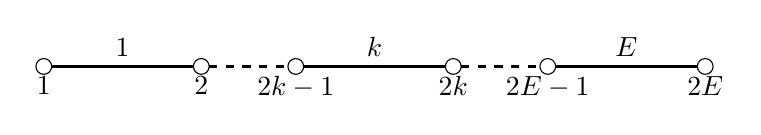
\begin{tikzpicture}
  \draw (2.3,0) circle (0.1) node [below] {$1$};
  \draw (4.3,0) circle (0.1) node [below] {$2$};
  \draw[thick] (2.4,0) -- (4.2,0) node [above,midway] {$1$};
  \draw[thick,dashed] (4.4,0) -- (5.4,0);
  \draw (5.5,0) circle (0.1) node [below] {$2k-1$};
  \draw (7.5,0) circle (0.1) node [below] {$2k$};
  \draw[thick] (5.6,0) -- (7.4,0) node [above,midway] {$k$};
  \draw[thick,dashed] (7.6,0) -- (8.6,0);
  \draw (8.7,0) circle (0.1) node [below] {$2E-1$};
  \draw (10.7,0) circle (0.1) node [below] {$2E$};
  \draw[thick] (8.8,0) -- (10.6,0) node [above,midway] {$E$};
\end{tikzpicture}

  \caption{One-dimensional mesh made of $E$ elements of constant length $\Delta x = \frac{l}{E}$.}\label{fig:1Dmesh}
\end{figure}
In that mesh, the cell containing the particle $I$ is denoted by $c(I)$ so that the nodes interacting with this particle are $2c(I)-1$ and $2c(I)$.
Since only scalar quantities are considered here, subscript can be used to denote nodal or particle values without ambiguity.
Therefore, the linear shape functions defined in element $c(I)$ are:
\begin{equation}
S_{2c(I)-1}(x)= \frac{x_{2c(I)} - x}{\Delta x} \: ; \: S_{2c(I)}(x)= \frac{x -x_{2c(I)-1}}{\Delta x} \quad x \in \[x_{2c(I)-1},x_{2c(I)}\]
\end{equation}
and $S_{iI}$ or $S_{i,I}$ correspond to the shape function of node $i$ evaluated at the position of the $I$th material point.
In order to better distinguish nodal and particle fields, uppercase symbols are used for material point quantities.

\subsection{The scheme equation}
The method followed to write the scheme equation is to trace backward the numerical procedure described in section \ref{sec:dgmpm} to get an expression of the form:
\begin{equation}
  \label{eq:scheme_general}
  \bar{Q}^{k+1}_I=H\(\bar{Q}^{k}_J\) \qquad  J=1,..,N_p
\end{equation}
where $H$ stands for the DGMPM discrete solution operator.

The two stages of the RK2 algorithm can be written as:
\begin{equation}
  \label{eq:RK2_algo}
  \bar{q}^{k+\frac{p+1}{2}}_i  =\bar{q}^{k}_i + \frac{p+1}{2}\frac{\Delta t}{M^L_{i}} s_1 \( \sum_{j=1}^{2E} K_{i,j} \bar{q}^{k+\frac{p}{2}}_j - \hat{F}^{k+\frac{p}{2}}_in_i \), \quad  \text{no sum on $i$}   
\end{equation}
in which $\hat{F}^{k+\frac{p}{2}}_i$ and $n_i=\pm1$ are respectively the intercell flux and the outward unit normal at node $i$, and $p=\{0,1\}$ refers to the two stages of the scheme.
Moreover, the mass density is approximated on the grid as:
\begin{equation}
  \label{eq:grid_density}
  \rho(x) = \frac{M^L_{2c-1}+M^L_{2c}}{\Delta x} = \frac{\sum_{J=1}^{N_p^c} m_J}{\Delta x}, \quad x \in [x_{2c-1},x_{2c}]
\end{equation}
where $N_p^{c}$ is the number of particles in cell $c$.
The mass is uniformly distributed between particles so that the previous definition reduces to $\rho = N_p^{c} m^c/\Delta x$, with $m^c$ the mass carried by particles lying in $c$.

First, quantities at time $t^{k+1}$ at particles are obtained by interpolating nodal solutions of the discrete system \eqref{eq:RK2_algo}: 
\begin{equation}
\bar{Q}^{k+1}_I = S_{2c(I)-1,I}\bar{q}_{2c(I)-1}^{k+1} + S_{2c(I),I}\bar{q}_{2c(I)}^{k+1} \label{eq:updated_MP}
\end{equation}
Second, provided linear shape functions, the lumped mass and the pseudo-stiffness matrices are:
\begin{align}
  & M^L_i = \sum_{J=1}^{N_p} S_{iJ} m_J = m^{c(i)} \sum_{J=1}^{N_p} S_{iJ}\\
  & K_{2c(I)-1,j} = \sum_{J=1}^{N_p} \drond{S_{2c(I)-1,J}}{x} m_J S_{jJ} = -m^{c(i)} \sum_{J=1}^{N_p} \frac{ S_{jJ}}{\Delta x} \\
  & K_{2c(I),j} = \sum_{J=1}^{N_p} \drond{S_{2c(I),J}}{x} m_J S_{jJ} = m^{c(i)}\sum_{J=1}^{N_p} \frac{ S_{jJ}}{\Delta x} 
\end{align}
The discontinuous approximation basis moreover yields a bloc diagonal pseudo-stiffness matrix so that one can write:
\begin{equation}
  \label{eq:block_diag_K}
  K_{ij} \bar{q}_{j}^{k}= K_{i,2c(i)-1} \bar{q}_{2c(i)-1}^{k}+K_{i,2c(i)} \bar{q}_{2c(i)}^{k}
\end{equation}
Third, a right-going wave leads to a stationary solution of Riemann problems equals to the state of the upwind node of an interface, that is:
\begin{align}
  & q_{2c(I)-1}^* = \rho \bar{q}^k_{2c(I)-2}=  N_p^{c(I)}\frac{ m^{c(I)}}{\Delta x}\bar{q}^k_{2c(I)-2} \\
  & q_{2c(I)}^* = \rho \bar{q}^k_{2c(I)} =  N_p^{c(I)}\frac{ m^{c(I)}}{\Delta x} \bar{q}^k_{2c(I)} 
\end{align}
Therefore, gathering all the previous considerations, equation \eqref{eq:RK2_algo} reads for each node of cell $c(I)$:
\begin{equation}
  \label{eq:nodal_RK2}
  \begin{aligned}
    & \bar{q}_{2c(I)-1}^{k+\frac{p+1}{2}}= \bar{q}_{2c(I)-1}^{k} - \frac{p+1}{2}\frac{s_1\Delta t}{\Delta x}\( \frac{f_{c(I)}^{k+\frac{p}{2}} - N_p^{c( I)} \bar{q}^{k+\frac{p}{2}}_{2c(I)-2}}{\sum_{K=1}^{N_p^{c(I)}}S_{2c(I)-1,K}}\)\\
    & \bar{q}_{2c(I)}^{k+\frac{p+1}{2}}= \bar{q}_{2c(I)}^{k} + \frac{p+1}{2}\frac{s_1\Delta t}{\Delta x}\( \frac{f_{c(I)}^{k+\frac{p}{2}} - N_p^{c( I)} \bar{q}^{k+\frac{p}{2}}_{2c(I)}}{\sum_{K=1}^{N_p^{c(I)}}S_{2c(I),K}}\)
    % & \bar{q}_{2c(\alpha)-1}^{k+(k+1)/2}= \bar{q}_{2c(\alpha)-1}^{k+k/2} - \frac{k+1}{2}\frac{a\Delta t}{\Delta x}\( \frac{\sum_{\mu=1}^{N_p^{c(\alpha)}} \[S_{2c(\alpha)-1,\mu}\bar{q}_{2c(\alpha)-1}^{k+k/2}+ S_{2c(\alpha),\mu}\bar{q}_{2c(\alpha)}^{k+k/2}\] - N_p^{c( \alpha)} \bar{q}^{k+k/2}_{2c(\alpha)-2}}{\sum_{\mu=1}^{N_p^{c(\alpha)}}S_{2c(\alpha)-1,\mu}}\)\\
    % & \bar{q}_{2c(\alpha)}^{k+(k+1)/2}= \bar{q}_{2c(\alpha)}^{k+k/2} - \frac{k+1}{2}\frac{a\Delta t}{\Delta x}\( \frac{\sum_{\mu=1}^{N_p^{c(\alpha)}} \[S_{2c(\alpha)-1,\mu}\bar{q}_{2c(\alpha)-1}^{k+k/2}+ S_{2c(\alpha),\mu}\bar{q}_{2c(\alpha)}^{k+k/2}\] - N_p^{c( \alpha)} \bar{q}^{k+k/2}_{2c(\alpha)}}{\sum_{\mu=1}^{N_p^{c(\alpha)}}S_{2c(\alpha),\mu}}\)
  \end{aligned},\quad p=\{0,1\}
\end{equation}
with the volume fluxes contributions $f_{c}^{k}=\sum_{J=1}^{N_p^{c}} \[S_{2c-1,J}\bar{q}_{2c-1}^{k}+ S_{2c,J}\bar{q}_{2c}^{k}\]$.
Note that equation \eqref{eq:nodal_RK2} involves the Courant number $s_1\Delta t/\Delta x$.

The first stage of equation \eqref{eq:nodal_RK2} (\textit{i.e. }$p=0$) yields the intermediate nodal fields in cell $c(I)$:
\begin{equation}
  \label{eq:discrete_RK2_step1}
  \begin{aligned}
    &\bar{q}_{2c(I)-1}^{k+\frac{1}{2}}= \bar{q}_{2c(I)-1}^{k} - \frac{s_1\Delta t}{2\Delta x}\( \frac{f_{c(I)}^{k} - N_p^{c( I)} \bar{q}^k_{2c(I)-2}}{\sum_{K=1}^{N_p^{c(I)}}  S_{2c(I)-1,K}}\)\\
    &\bar{q}_{2c(I)}^{k+\frac{1}{2}}= \bar{q}_{2c(I)}^{k} + \frac{s_1\Delta t}{2\Delta x}\( \frac{f_{c(I)}^{k}- N_p^{c( I)}  \bar{q}^k_{2c(I)}}{\sum_{K=1}^{N_p^{c(I)}}  S_{2c(I),K}} \)
  \end{aligned}
\end{equation}
and the second one (\textit{i.e. }$p=1$) leads to the expression of nodal quantities at the end of the time step:
\begin{equation}
  \label{eq:discrete_RK2_step2}
  \begin{aligned}
    &\bar{q}_{2c(I)-1}^{k+1}= \bar{q}_{2c(I)-1}^{k} - \frac{s_1\Delta t}{\Delta x}\( \frac{\sum_{J=1}^{N_p^{c(I)}}\[S_{2c(I)-1,J}\bar{q}_{2c(I)-1}^{k+\frac{1}{2}}+ S_{2c(I),J}\bar{q}_{2c(I)}^{k+\frac{1}{2}}\] - N_p^{c( I)} \bar{q}^{k+\frac{1}{2}}_{2c(I)-2}}{\sum_{K=1}^{N_p^{c(I)}}  S_{2c(I)-1,K}}\)\\
    &\bar{q}_{2c(I)}^{k+1}= \bar{q}_{2c(I)}^{k} + \frac{s_1\Delta t}{\Delta x}\( \frac{\sum_{J=1}^{N_p^{c(I)}}\[S_{2c(I)-1,J}\bar{q}_{2c(I)-1}^{k+\frac{1}{2}}+ S_{2c(I),J}\bar{q}_{2c(I)}^{k+\frac{1}{2}}\]- N_p^{c( I)}  \bar{q}^{k+\frac{1}{2}}_{2c(I)}}{\sum_{K=1}^{N_p^{c(I)}}  S_{2c(I),K}} \)
  \end{aligned}
\end{equation}
Then, introduction of equations \eqref{eq:discrete_RK2_step2} in the interpolation from nodes to particles \eqref{eq:updated_MP} leads to the solution at material point $I$ and time step $k+1$:
\begin{equation}
  \label{eq:second_stage_MP}
  \begin{split}
    \bar{Q}^{k+1}_I &=  S_{2c(I)-1,I}\bar{q}_{2c(I)-1}^{k}+S_{2c(I),I}\bar{q}_{2c(I)}^{k} +N_p^{c(I)}\frac{s_1\Delta t}{\Delta x}\frac{S_{2c(I)-1,I}}{\sum_{K}  S_{2c(I)-1,K}}\bar{q}_{2c(I)-2}^{k+\frac{1}{2}} \\
    &- \(\frac{s_1\Delta t}{\Delta x}\[S_{2c(I)-1,I} - S_{2c(I),I}\frac{\sum_{J} S_{2c(I)-1,J}}{\sum_{K}  S_{2c(I),K}}\] \)\bar{q}_{2c(I)-1}^{k+\frac{1}{2}} \\
    & + \frac{s_1\Delta t}{\Delta x}\[S_{2c(I),I} - S_{2c(I)-1,I}\frac{\sum_{J} S_{2c(I),J}}{\sum_{K}  S_{2c(I)-1,K}}- N_p^{c(I)}\frac{S_{2c(I),I}}{\sum_{K}  S_{2c(I),K}}\] \bar{q}_{2c(I)}^{k+\frac{1}{2}}
  \end{split}
\end{equation}
Nodal values $\bar{q}_i^{k+\frac{1}{2}}$ are provided by the first stage of RK2 algorithm and can be substituted the above equation: %in equation \eqref{eq:second_stage_MP}:
\begin{equation}
  \begin{split}
    \bar{Q}^{k+1}_I &=  S_{2c(I)-1,I}\bar{q}_{2c(I)-1}^{k} +S_{2c(I),I}\bar{q}_{2c(I)}^{k} +N_p^{c(I)}\frac{s_1\Delta t}{\Delta x}\frac{S_{2c(I)-1,I}}{\sum_{K}  S_{2c(I)-1,K}}\(\bar{q}_{2c(I)-2}^{k} + \frac{s_1\Delta t}{2\Delta x}\( \frac{f_{c(I)-1}^{k}- N_p^{c( I)}  \bar{q}^k_{2c(I)-2}}{\sum_{K}  S_{2c(I)-2,K}} \)\)\\
    -& \frac{s_1\Delta t}{\Delta x}\[S_{2c(I)-1,I} - S_{2c(I),I}\frac{\sum_{J} S_{2c(I)-1,J}}{\sum_{K}  S_{2c(I),K}}\] \(\bar{q}_{2c(I)-1}^{k} - \frac{s_1\Delta t}{2\Delta x}\( \frac{f_{c(I)}^{k} - N_p^{c( I)} \bar{q}^k_{2c(I)-2}}{\sum_{K}  S_{2c(I)-1,K}}\)\) \\
    +& \frac{s_1\Delta t}{\Delta x}\[S_{2c(I),I}\(1- \frac{N_p^{c(I)}}{\sum_{K}  S_{2c(I),K}}\) - S_{2c(I)-1,I}\frac{\sum_{J} S_{2c(I),J}}{\sum_{K}  S_{2c(I)-1,K}}\] \(\bar{q}_{2c(I)}^{k} + \frac{s_1\Delta t}{2\Delta x}\( \frac{f_{c(I)}^{k}- N_p^{c( I)}  \bar{q}^k_{2c(I)}}{\sum_{K}  S_{2c(I),K}} \)\)
    \label{eq:Mp_before_mapping}
  \end{split}
\end{equation}
Note that the solution of the downstream node of the adjacent cell $\bar{q}^{k+\frac{1}{2}}_{2c(I)-2}$ results from the second equation of the set \eqref{eq:discrete_RK2_step1}.
Therefore, by rearranging formula \eqref{eq:Mp_before_mapping}:
%Note that the second equation of the set \eqref{eq:discrete_RK2_step1} is used for $q^{k+\frac{1}{2}}_{2c(J)-2}$ since it is the downwstream node of the adjacent cell $c(J)-1$. At last, by rearranging formula \eqref{eq:Mp_before_mapping} as:
\begin{equation}
  \label{eq:euler_before_mapping}
  \begin{split}
    \bar{Q}^{k+1}_I =  &\(S_{2c(I)-1,I} -\frac{s_1\Delta t}{\Delta x}\[S_{2c(I)-1,I} - S_{2c(I),I}\frac{\sum_{J} S_{2c(I)-1,J}}{\sum_{K}  S_{2c(I),K}}\]\)\bar{q}_{2c(I)-1}^{k} \\
    +&\(S_{2c(I),I} + \frac{s_1\Delta t}{\Delta x}\[S_{2c(I),I}\(1-\frac{N_p^{c(I)}}{\sum_{K}  S_{2c(I),K}}\) - S_{2c(I)-1,I}\frac{\sum_{J} S_{2c(I),J}}{\sum_{K}  S_{2c(I)-1,K}}\]\) \bar{q}_{2c(I)}^{k} \\
    +&\frac{1}{2}\(\frac{s_1\Delta t}{\Delta x}\)^2\(N_p^{c( I)}\[\frac{S_{2c(I)-1,I}}{\sum_K S_{2c(I)-1,K}} - \frac{S_{2c(I),I}}{\sum_{K}  S_{2c(I),K}}\] +S_{2c(I),I} \(\frac{N_p^{c(I)}}{\sum_{K}  S_{2c(I),K}}\)^2\)\bar{q}_{2c(I)}^{k}\\
    +&N_p^{c( I)}\frac{s_1\Delta t}{\Delta x}  \[ \frac{S_{2c(I)-1,I}}{\sum_{K}  S_{2c(I)-1,K}}\(1 -   \frac{s_1\Delta t}{2\Delta x}\(1+\frac{N_p^{c( I)} }{\sum_{K}  S_{2c(I)-2,K}} \)\)+\frac{s_1\Delta t}{2\Delta x} \frac{S_{2c(I),I}}{\sum_{K}  S_{2c(I),K}}\]\bar{q}^k_{2c(I)-2}\\
    -&\frac{1}{2}\(\frac{s_1\Delta t}{\Delta x}\)^2 N_p^{c(I)}\frac{S_{2c(I),I}}{\(\sum_{K}  S_{2c(I),K}\)^2} f_{c(I)}^{k} +\frac{1}{2}\(\frac{s_1\Delta t}{\Delta x}\)^2N_p^{c(I)}\frac{S_{2c(I)-1,I}}{\sum_{K}  S_{2c(I)-1,K}}\frac{ f_{c(I)-1}^{k}}{\sum_{K}  S_{2c(I)-2,K}}
  \end{split}
\end{equation}

Next, the nodal solutions at time step $k$ in equation \eqref{eq:euler_before_mapping} result from the projection between particles and the grid \eqref{eq:DGMPM_points2nodes}:
%In equation \eqref{eq:euler_before_mapping} the solutions at nodes result from the convection step \eqref{eq:DGMPM_points2nodes}:
\begin{equation}
\bar{q}^{k}_{i} = \frac{\sum_L S_{iL}m_L \bar{Q}^k_{L}}{\sum_K S_{iK}m_K} = \frac{\sum_L S_{iL} \bar{Q}^k_{L}}{\sum_K S_{iK}} \label{eq:stab_mapping}
\end{equation}
In particular, volume fluxes contributions can be written:
\begin{equation}
  \label{eq:volume_fluxes_mapped}
  \begin{aligned}
    f_{c}^{k}&=\sum_{J=1}^{N_p^{c}}\[S_{2c-1,J}\frac{\sum_L S_{2c-1,L}\bar{Q}^k_{L}}{\sum_K S_{2c-1,K}}+ S_{2c,J}\frac{\sum_L S_{2c,L} \bar{Q}^k_{L}}{\sum_K S_{2c,K}} \]\\
    f_{c}^{k}&=\sum^{N_p}_{L=1}\(S_{2c-1,L} +S_{2c,L} \)\bar{Q}^k_{L}  \\ 
    f_{c}^{k}&=\sum^{}_{L \in c}\bar{Q}^k_{L}   
  \end{aligned}
\end{equation}
where the partition of unity yields the last equality.

The use of mapping equations \eqref{eq:stab_mapping} and \eqref{eq:volume_fluxes_mapped} allows to write after some simplifications:
% \begin{equation}
%   \begin{split}
%     \bar{Q}^{k+1}_I =  &\sum_{L} \bar{Q}_L^k  \left\lbrace \frac{S_{2c(I)-1,L}}{\sum_K S_{2c(I)-1,K}}\(S_{2c(I)-1,I} -\frac{s_1\Delta t}{\Delta x}\[S_{2c(I)-1,I} - S_{2c(I),I}\frac{\sum_{J} S_{2c(I)-1,J}}{\sum_{K}  S_{2c(I),K}}\]\)  \right. \\
%     &+\frac{S_{2c(I),L}}{\sum_K S_{2c(I),K}}\(S_{2c(I),I} + \frac{s_1\Delta t}{\Delta x}\[S_{2c(I),I}\(1-\frac{N_p^{c(I)}}{\sum_{K}  S_{2c(I),K}}\) - S_{2c(I)-1,I}\frac{\sum_{J} S_{2c(I),J}}{\sum_{K}  S_{2c(I)-1,K}}\]\)  \\
%     &+\frac{S_{2c(I),L}}{\sum_K S_{2c(I),K}}\frac{1}{2}\(\frac{s_1\Delta t}{\Delta x}\)^2\(N_p^{c(I)}\[\frac{S_{2c(I)-1,I}}{\sum_K S_{2c(I)-1,K}} - \frac{S_{2c(I),I}}{\sum_{K}  S_{2c(I),K}}\] +S_{2c(I),I} \(\frac{N_p^{c(I)}}{\sum_{K}  S_{2c(I),K}}\)^2\)  \\
%     &+\frac{N_p^{c(I)} S_{2c(I)-2,L}}{\sum_K S_{2c(I)-2,K}}\frac{s_1\Delta t}{\Delta x} \[ \frac{S_{2c(I)-1,I}}{\sum_{K}  S_{2c(I)-1,K}}\(1 -   \frac{s_1\Delta t}{2\Delta x}\(1+\frac{N_p^{c(I)} }{\sum_{K}  S_{2c(I)-2,K}} \)\)+\frac{s_1\Delta t}{2\Delta x} \frac{S_{2c(I),I}}{\sum_{K}  S_{2c(I),K}}\]\\
%     &+\frac{1}{2}\(\frac{s_1\Delta t}{\Delta x}\)^2 N_p^{c(I)}\left.\( \frac{S_{2c(I)-2,L} +S_{2c(I)-3,L} }{\sum_{K}  S_{2c(I)-1,K}\sum_{K}  S_{2c(I)-2,K}} S_{2c(I)-1,I}-\frac{S_{2c(I)-1,L} +S_{2c(I),L} }{\(\sum_{K}  S_{2c(I),K}\)^2} S_{2c(I),I}\)  \right\rbrace
%   \end{split}
% \end{equation}
% Once the previous formula is simplified, the one-dimensional scheme equation of the DGMPM with the RK2 time discretization can be written:
\begin{equation}
  \label{eq:RK2_scheme}
  \begin{split}
    \bar{Q}^{k+1}_I =  &\sum_{L} \bar{Q}_L^k  \left\lbrace \sum_i S_{iL}\frac{S_{iI}}{\sum_K S_{iK}}
      +\frac{s_1\Delta t}{\Delta X}\[\frac{S_{2c(L),I}}{\sum_{K}  S_{2c(L),K}} - \frac{S_{2c(L)-1,I}}{\sum_{K}  S_{2c(L)-1,K}}\] \right.\\
    &+\frac{s_1\Delta t}{\Delta X}N_p^{c( I)}\[\frac{S_{2c(I)-1,I}}{\sum_{K}  S_{2c(I)-1,K}}\frac{S_{2c(I)-2,L}}{\sum_K S_{2c(I)-2,K}}-\frac{S_{2c(I),I}S_{2c(I),L}}{\(\sum_K S_{2c(I),K}\)^2}\] \\
    &+\frac{1}{2}\(\frac{s_1\Delta t}{\Delta X}\)^2N_p^{c( I)} \(\frac{S_{2c(I),L}}{\sum_K S_{2c(I),K}}-\frac{S_{2c(I)-2,L}}{\sum_K S_{2c(I)-2,K}}\)\[\frac{S_{2c(I)-1,I}}{\sum_K S_{2c(I)-1,K}} - \frac{S_{2c(I),I}}{\sum_{K}  S_{2c(I),K}}\]\\
    &+\frac{1}{2}\(\frac{s_1\Delta t}{\Delta X}\)^2N_p^{c( I)}\frac{S_{2c(L),I}}{\(\sum_{K}  S_{2c(I),K}\)^2} \[N_p^{c( I)}\frac{S_{2c(I),L} }{\sum_K S_{2c(I),K}}-1\]\\
    &+ \frac{1}{2}\(\frac{s_1\Delta t}{\Delta X}\)^2\frac{S_{2c(L)+1,I}N_p^{c(I)}}{\sum_{K}  S_{2c(I)-1,K}\sum_{K}  S_{2c(I)-2,K}} \left.\[ 1 - N_p^{c( I)}\frac{S_{2c(I)-2,L} }{\sum_{K}  S_{2c(I)-2,K}}\] \right\rbrace
    \end{split}
\end{equation}
The three first terms of the latter scheme equation correspond to that obtained for the Euler algorithm \cite{DGMPM}, whereas the second-order terms are provided by the two-stage time integration.
% The brackets in those higher-order corrections vanish when only one point is in each cell of the grid, so that the scheme is equivalent to the well-known first-order upwind method. %% Add comments
% This property of the DGMPM has already been observed for the Euler time discretization \cite{DGMPM}.
Alternatively and given the compact support of shape functions, equation \eqref{eq:RK2_scheme} can be split into two sums, one over the material points contained in the cell $c(I)$, and one over these of cell $c(I)-1$:
\begin{equation}
  \label{eq:RK2_scheme_split}
  \begin{split}
    \bar{Q}^{k+1}_I &=  \sum_{L\in c(I)} \bar{Q}_L^k  \left\lbrace \sum_i S_{iL}\frac{S_{iI}}{\sum_K S_{iK}}
      +\frac{s_1\Delta t}{\Delta X}\[\frac{S_{2c(L),I}}{\sum_{K}  S_{2c(L),K}} - \frac{S_{2c(L)-1,I}}{\sum_{K}  S_{2c(L)-1,K}} - N_p^{c( I)}\frac{S_{2c(I),I}S_{2c(I),L}}{\(\sum_K S_{2c(I),K}\)^2}\] \right.\\
    &\left.+\frac{1}{2}\(\frac{s_1\Delta t}{\Delta X}\)^2N_p^{c( I)} \frac{S_{2c(I),L}}{\sum_K S_{2c(I),K}}\[\frac{S_{2c(I)-1,I}}{\sum_K S_{2c(I)-1,K}} - \frac{S_{2c(I),I}}{\sum_{K}  S_{2c(I),K}}+ N_p^{c( I)}\frac{S_{2c(I),L} }{\(\sum_K S_{2c(I),K}\)^2}-\frac{1}{\sum_K S_{2c(I),K}}\]\right\rbrace\\
    %%%% OTHER SUM
    &+ \sum_{L\in c(I)-1} \bar{Q}_L^k  N_p^{c( I)}\left\lbrace  
      \frac{s_1\Delta t}{\Delta X}\frac{S_{2c(I)-1,I}}{\sum_{K}  S_{2c(I)-1,K}}\frac{S_{2c(L),L}}{\sum_K S_{2c(L),K}} \right. \\
    % &-\frac{1}{2}\(\frac{s_1\Delta t}{\Delta X}\)^2 \frac{S_{2c(L),L}}{\sum_K S_{2c(L),K}}\[\frac{S_{2c(I)-1,I}}{\sum_K S_{2c(I)-1,K}} - \frac{S_{2c(I),I}}{\sum_{K}  S_{2c(I),K}}\]\\
    % &+ \frac{1}{2}\(\frac{s_1\Delta t}{\Delta X}\)^2\frac{S_{2c(L)+1,I}}{\sum_{K}  S_{2c(I)-1,K}} \left.\[\frac{ 1}{\sum_{K}  S_{2c(L),K}} - \frac{S_{2c(L),L} N_p^{c( I)}}{\(\sum_{K}  S_{2c(L),K}\)^2}\] \right\rbrace
    %% TEST FOR LAST TWO LINES
    & \left.+ \frac{1}{2}\(\frac{s_1\Delta t}{\Delta X}\)^2\(\frac{S_{2c(L)+1,I}}{\sum_{K}  S_{2c(I)-1,K}} \[\frac{ 1}{\sum_{K}  S_{2c(L),K}} - \frac{S_{2c(L),L} N_p^{c( I)}}{\(\sum_{K}  S_{2c(L),K}\)^2}\]-\frac{S_{2c(L),L}}{\sum_K S_{2c(L),K}}\[\frac{S_{2c(I)-1,I}}{\sum_K S_{2c(I)-1,K}} - \frac{S_{2c(I),I}}{\sum_{K}  S_{2c(I),K}}\]\)\right\rbrace
    \end{split}
\end{equation}
When only one point lies in each cell of the grid, the sum of shape functions over particles reduces to one single term (\textit{e.g. }$\sum_{K}  S_{2c(J)-1,K} = S_{2c(J)-1,J}$).
Thus, one can show that the terms under brackets in the above equation all vanish so that the scheme reduces to:
\begin{equation}
  \label{eq:RK2_1ppc}
  \bar{Q}^{k+1}_I=  (1-\frac{s_1\Delta t}{\Delta X})\bar{Q}_I^k+\frac{s_1\Delta t}{\Delta X}\bar{Q}_{I-1}^k
\end{equation}
%which corresponds to the well-known first-order upwind method.
It then appears that, as for the DGMPM combined with the Forward Euler time integration \cite{DGMPM}, the use of one particle per cell and RK2 time discretization within the DGMPM leads, for one-dimensional problems, to the well-known first-order upwind method.
%Thus, assuming that the approximation leads to an order of accuracy greater than one, a first-order of accuracy can be achieved by adapting only the space discretization and the polynomial order.
%This is an interesting feature of the scheme in order to capture discontinuities.
% This result highlights an interesting feature of the DGMPM which consists in allowing to modify the order of the method by only changing the space discretization.
%Indeed, assuming that the approximation leads to an order of accuracy greater than one, the use of only one particle and linear shape functions in a cell enables to locally achieve first order accuracy even for a second-order time integration.
%Hence, if the cell is known to be crossed by a discontinuity, the required first-order can be reached so as to capture the jump.

\subsection{The von Neumann linear stability analysis}

The scheme equation \eqref{eq:RK2_scheme} is written for simplicity:
\begin{equation}
\bar{Q}^{k+1}_I = \sum_{L=1}^{N_p}  H_{IL} \bar{Q}^k_{L}\label{eq:scheme_Dpi}
\end{equation}
Moreover, the computational domain is repeated periodically by mapping it to the domain $[-l,0]$ so that the solution at material point $I$ and time step $k$ is expanded into a discrete Fourier basis of $2E+1$ harmonics over the domain $x \in \[-l,l\]$:
\begin{equation}
\bar{Q}^{k}_I = \sum_{j=-E}^{E}A_j^k e^{i I \lambda_j \Delta x}
\end{equation}
with $A^k_j$, the magnitude of the $j$th harmonic at time step $k$, $i = \sqrt{-1}$, and $\lambda_j$ the wave number.
Introduction of this expansion in equation \eqref{eq:scheme_Dpi} yields:
\begin{equation}
A_j^{k+1} e^{iI \lambda_j \Delta x} = \sum_{L=1}^{N_p} A_j^k H_{IL}e^{i L \lambda_j \Delta x}\quad \forall j=-E,...,E
\end{equation}
The amplification factor between two time steps at a given point is defined as:
\begin{equation}
\frac{A_j^{k+1}}{A_j^k} = \sum_{L=1}^{N_p} e^{i (L -I)\lambda_j \Delta x} H_{IL} \quad \forall j=-E,...,E \label{eq:fourier_expansion}
\end{equation}
A necessary condition to ensure the stability of a numerical scheme is that the amplification factor must be lower than or equal to one in modulus: $\abs{A^{k+1}/A^k} \leq 1$.
This upper bound allows to prevent an increasing error during the computation. For expression \eqref{eq:fourier_expansion}, this leads to:
\begin{equation}
 \abs{\sum_{L=1}^{N_p} e^{i (L -I)\lambda_j \Delta x} H_{IL}} \leq \sum_{L=1}^{N_p} \abs{e^{i (L -I)\lambda_j \Delta x} H_{IL}} = \sum_{L=1}^{N_p} \abs{H_{IL}} \quad \forall j=-E,...,E
\end{equation}
where the triangle inequality, and the unit modulus of the complex number $e^{i (L -I)\lambda_j \Delta x}$ have been used.
Hence, the DGMPM scheme is stable for a given discretization if the Courant number is set so that the following condition is satisfied for all material points:
\begin{equation}
  \label{eq:stability} \sum_{L=1}^{N_p} \abs{H_{IL}} \leq 1 \quad \forall \: I = 1,...,N_p
\end{equation}
The stability of the scheme is thus ensured by using the lowest CFL number satisfying \eqref{eq:stability}.
Note however that the use of the triangle inequality leads to a more severe constraint than that really admissible.
As a consequence, the Courant number can be set in practice to higher values than that resulting from the solution of \eqref{eq:stability}. 

\subsection{Evaluation of the CFL number for particular space discretizations}
%According to the scheme equation \eqref{eq:RK2_scheme},

The stability condition \eqref{eq:stability} can be very hard to solve analytically for general discretizations.
Nevertheless, the Courant number can be set to unity for one particle lying in every cells, regardless of their positions, since in that case the DGMPM scheme identifies to the first-order upwind method.
On the other hand, though the infinity of possible material points distributions prevents the explicit derivation of a general stability condition, the optimal CFL number satisfying the equality in \eqref{eq:stability} can be found numerically.
Some configurations are studied in table \ref{tab:CFL_comparison} where the critical Courant number resulting from the two time discretizations studied above are compared.
Those results have been obtained by using the same particles distribution in every elements of a one-dimensional regular mesh. 
%
The following configurations are considered:
\begin{itemize}
\item[(i)] particles are positioned symmetrically with respect to cells centers and regularly spaced in the mesh. This space discretization is referred to as the natural configuration in the following.
\item[(ii)] particles in the natural configuration are all shifted of $u=\Delta x/10$.
\item[(iii)] the same than (ii) with $u$ so that one material point overlaps every left nodes of cells.
\item[(iv)] the same than (iii) for right nodes.
\item[(v)] particles are placed symmetrically with respect to cells centers but not regularly spaced in the mesh. Material points in the left half of cells are shifted of $u_1=-\Delta x/10$ while those in the right half are shifted of $u_2=\Delta x/10$.
\item[(vi)] the same than (v) with the first and last particles overlapping left and right nodes of cells respectively.
\end{itemize}


\begin{table}[h!]
  \centering
  \begin{tabular}[ht]{cccccN}
  \hline
  \multicolumn{2}{c}{Number of particles} & Position of $I$th particle in cell $c$ & Euler CFL & RK2 CFL &\\[6pt]
  \hline
  \hline
  (--) &1 &$X^1 \in \[X^{2c-1},X^{2c}\]$  &  1 & 1&\\[8pt]
  \hline
  (i)& 2 & $ X^I= X^{2c-1}+(2I-1)\frac{\Delta X}{4}$ &  0.43 & 1&\\[8pt]
  (ii)& 2 & $X^I= X^{2c-1}+(2I-1)\frac{\Delta X}{4} +\frac{\Delta X}{10} $ &  0.40 & 0.50 &\\[8pt]
  (iii)& 2 & $X^I= X^{2c-1}+(2I-1)\frac{\Delta X}{4} +(I-2)\frac{\Delta X}{10} $ &  0.27 & 1 &\\[8pt]
  (iii)'& 2 & $X^I= X^{2c-1}+(2I-1)\frac{\Delta X}{4} +(I-2)\frac{\Delta X}{4} $ &  0 & 1 &\\[8pt]
  \hline
  (i)& 3 & $ X^I= X^{2c-1}+2I\frac{\Delta X}{8}$ &  0.43 & 1&\\[8pt]
  (ii)& 3 & $X^I= X^{2c-1}+2I\frac{\Delta X}{8} +\frac{\Delta X}{10} $ &  0.40 & 0.50 &\\[8pt]
  (iii)& 3 & $X^I= X^{2c-1}+2I\frac{\Delta X}{8} +(I-2)\frac{\Delta X}{10} $ &  0.27 & 1 &\\[8pt]
  (iii)'& 3 & $X^I= X^{2c-1}+2I\frac{\Delta X}{8} +(I-2)\frac{\Delta X}{4} $ &  0 & 1 &\\[8pt]
  \hline
  (i)& 4 & $ X^I= X^{2c-1}+I\frac{\Delta X}{5}$ &  0.35 & 1&\\[8pt]
  (ii)& 4 & $X^I= X^{2c-1}+I\frac{\Delta X}{5} +\frac{\Delta X}{10} $ &  0.31 & 0.40 &\\[8pt]
  (iii)& 4 & $X^I= X^{2c-1}+I\frac{\Delta X}{5} +\frac{2I-5}{\abs{2I-5}}\frac{\Delta X}{10} $ &  0.18 & 1 &\\[8pt]
  (iii)'& 4 & $X^I= X^{2c-1}+I\frac{\Delta X}{5} +\frac{2I-5}{\abs{2I-5}}\frac{\Delta X}{5} $ &  0 & 1 &\\[8pt]
  \hline
\end{tabular}

%%% Local Variables: 
%%% mode: latex
%%% TeX-master: "../../mainManuscript"
%%% End:
  \caption{DGMPM critical Courant number values for Euler or RK2 time integration for several one-dimensional discretizations. Black circles denote material points while white ones represent grid nodes.}
  \label{tab:CFL_comparison}
\end{table}
First, table \ref{tab:CFL_comparison} shows that the natural configuration leads to the optimal stability bound for the RK2 integrator while the CFL number allowed by using Euler time discretization decreases with increasing number of particles per cell.
Second, moving every points rightward in the mesh (\textit{i.e. cases (ii) and (iv)}) causes a drop in the critical Courant number for both RK2 and Euler algorithms. In particular, stability conditions for more than two particles per cell provided by the RK2 are, in those cases, more restrictive than that of the Euler.
Third, the leftward shifting (\textit{i.e. case (iii)}) leads on the other hand to an improvement of the stability condition for Euler time integration compared to that enabled in the natural configuration.
This property illustrates the upwind nature of the scheme since $s_1>0$.
The CFL number provided by RK2 integration also decreases due to the shifting while remaining higher than Euler one.
At last, particles distributions conserving the symmetry with respect to cells centers (\textit{i.e. cases (v) and (vi)}), yield the optimal stability condition for the RK2 integrator while the Euler CFL depends on the spacing between material points.
More specifically, Euler algorithm leads to a vanishing CFL for the case (vi), thus preventing any simulation.

% Comparison with DGFEM
%\note{2) According to the reviewer "the critical Courant number being similar to the Eulerian DG schemes despite the Lagrangian aspect", make sure that it is true...}
\review{
  Notice that although the stability depends on the position of particles, the optimal Courant number can be reached even with the Euler discretization, whereas the classical DGFEM scheme presented in  \cite{Chavent_Salzano} is restricted to condition $\Delta t / \Delta x = \mathcal{O}(\sqrt{\Delta x})$.
  This limitation has been addressed by introducing slope limiters in order to remove non-physical oscillations in the vicinity of sharp solutions while providing high-order accuracy in smooth regions \cite{Chavent_Cockburn}.
  However, the stability of the method is still bounded by $CFL\leq 1/2$ and the scheme was first-order accurate.
  The use of a second-order Runge-Kutta \cite{DGFEM_CFL} allows to achieve second-order accuracy of the scheme, but the stability condition then reduces to $CFL\leq1/3$.
  It is noteworthy that space-time DGFEM formulations \cite{ST_DGFEM1,ST_DGFEM2} provided more recently the ability to relax constraints of pure space DGFEM and obtained a critical CFL set at 1.
  %
  % Given the applications aimed by the method, which involve discontinuities in finite-deforming solids, the stability properties of DGMPM and DGFEM schemes must be supplemented by the ability of the methods to handle large deformations for a complete comparison.
  % In that context, the DGMPM 
}
%%% Local Variables:
%%% mode: latex
%%% TeX-master: "manuscript"
%%% End:


\section{Stability properties of the two-dimensional schemes}
\label{sec:2d_stab}
\subsection{The scheme equation}
We now move on to the scalar linear advection equation with positive coefficients $s_1,s_2>0$.
Moreover, the space coordinates $x_1,x_2$ in the ($\vect{e}_1,\vect{e}_2$) plane are written $x$ and $y$.
Then, the physical domain under consideration, that is $x,y \in [0,l]\times[0,h]$, is discretized with $N_p$ material points arbitrarily distributed in a Cartesian grid made of $E$ four-node bilinear elements with constant size $\Delta x \times \Delta y$.
\begin{figure}[h!]
  \centering
  \begin{tikzpicture}
  \draw[thick,->] (-1.5,0.)--(1.5,0.) node [right] {$\xi$};
  \draw[thick,->] (0.,-1.5)--(0.,1.5) node [above] {$\eta$};
  \draw (-1.,-1.0) rectangle (1.,1.);
  \node[above right] at (0.,1.) {$1$};\node[above right] at (0.,-1.) {-$1$};
  \node[above right] at (-1,0.) {-$1$};\node[above right] at (1.,.) {$1$};
  \draw[thick,->] (-.25+5.,0.)--(1.5+5.,0.) node [right] {$X$};
  \draw[thick,->] (0.+5.,-.25)--(0.+5.,1.5) node [above] {$Y$};
  % origin at (+5.,0.)
  \draw (6.,1.) node [below] {$X_1$}-- (8.,1.5) node [below] {$X_2$}-- (9.,4.) node [above] {$X_3$}-- (6.5,3.5) node [above] {$X_4$}-- (6.,1.);
  \fill[black] (8.,3.25) circle (0.05) node [above] {$\vect{X}$};
  \fill[black] (.5,.5) circle (0.05) node [above] {$\vect{\xi}$};
  \draw[->] (8.,3.25) .. controls (6.,3.25) and (1.5,1.5) .. (.5,.5);
\end{tikzpicture}
  
  \caption{Parent and current configuration of a rectangular four-node bilinear element}
  \label{fig:2Dparent}
\end{figure}
With positions of nodes of cell $C$ denoted by $\vect{x}_i^C=\matrice{x^C_i \\ y_i^C}$, as depicted in figure \ref{fig:2Dparent}, the location $\vect{x}$ of an arbitrary point in cell $C$ maps to the parent coordinates $(\xi,\eta)$ in the domain $\[-1,1\]\times\[-1,1\]$ according to:
\begin{equation}
  \label{eq:parentCoordinates}
  \begin{aligned}
      &\xi = 2\frac{x-x^C_1}{\Delta x} -1 \quad ; \quad d\xi = 2\frac{dx}{\Delta x} \\
      &\eta = 2\frac{y-y^C_1}{\Delta y} -1 \quad ; \quad d\eta = 2\frac{dy}{\Delta y} 
  \end{aligned}
\end{equation}
Horizontal and vertical edges lengths are distinguished here in spite of the Cartesian nature of the grid in order to easily extend the following study to rectilinear grids. Again, there is no empty cell inside the physical domain so that no hole is generated, and periodic boundary conditions are considered to simplify the analysis.
Though, one can imagine to combine the DGMPM discretization with a multi-stage time integration as proposed for one-dimensional problems, the equations one has to deal with become complicated.
Hence, the analysis of the DGMPM scheme for two-dimensional problems carried out here only considers the Euler time discretization.

The updated solution at material point $I$ is obtained by interpolation of updated nodal quantities:
\begin{equation}
  \label{eq:2D_updatedMP}
  \bar{Q}^{k+1}_I = \sum_{i=1}^{4E}S_{iI} \bar{q}_i^{k+1}
\end{equation}
where the $\bar{q}_i^{k+1}$ result from the discrete system:
\begin{equation}
  \bar{q}_i^{k+1} = \bar{q}_i^k + \frac{\Delta t}{M^L_i} \(K_{ij}^x s_1\bar{q}_j^k + K_{ij}^y s_2\bar{q}_j^k - \hat{F}^k_i\) \label{eq:discrete2D}
\end{equation}

The lumped mass matrix in the above equation has the same expression as in the one-dimensional case that depends on the shape functions of the four-node bilinear element: $M_i^L=\sum_K m_K S_{iK}$.
Making use of parent coordinates \eqref{eq:parentCoordinates}, the pseudo-stiffness matrices read:
\begin{equation}
  \begin{aligned}
    & K_{ij}^x = \sum_J \drond{S_{iJ}}{x}m_J S_{jJ}=\frac{2}{\Delta x}\sum_J\drond{S_{iJ}}{\xi}m_J S_{jJ} \\
    &K_{ij}^y = \sum_J\drond{S_{iJ}}{y}m_J S_{jJ}=\frac{2}{\Delta y}\sum_J\drond{S_{iJ}}{\eta}m_J S_{jJ} \\
  \end{aligned}
\end{equation}
As for one-dimensional cases, the homogeneous medium yields the same mass for every particles so that, by writing $\drond{(\bullet)}{\xi}=\partial_\xi(\bullet)$, one gets:
\begin{equation}
  \label{eq:2Dpseudo_stiffness}
  \begin{aligned}
    & \frac{K_{ij}^x}{M_i^L}  =  \frac{2}{\Delta x} \frac{\sum_J\partial_\xi S_{iJ}  S_{jJ}}{\sum_K  S_{iK}} \\
    & \frac{K_{ij}^y}{M_i^L} = \frac{2}{\Delta y} \frac{\sum_J\partial_\eta S_{iJ} S_{jJ}}{\sum_K S_{iK}}
  \end{aligned}
\end{equation}
The nodal solutions in cell $C$ at time $k$ being given by the projection $\bar{q}^{C,k}_i=\frac{\sum_L S_{iL}\bar{Q}^k_L}{\sum_K S_{iK}}$, volume fluxes of the discrete form can be rewritten as:
\begin{equation}
  \label{eq:2Dvolume_fluxes}
  \begin{aligned}
    & s_1\frac{K_{ij}^x}{M_i^L}\bar{q}^k_j  = \sum_L\bar{Q}^k_L\frac{2}{\Delta x} \frac{s_1\sum_J\partial_\xi S_{iJ}  \sum_j S_{jJ} S_{jL}}{\sum_K S_{iK}\sum_K S_{jK}}\\
    & s_2\frac{K_{ij}^y}{M_i^L}\bar{q}^k_j = \sum_L \bar{Q}^k_L\frac{2}{\Delta y}  \frac{s_2 \sum_J\partial_\eta S_{iJ}  \sum_j S_{jJ} S_{jL}}{\sum_K  S_{iK}\sum_K S_{jK}}
  \end{aligned}
\end{equation}
Then, the nodal interface flux $\hat{F}^k_i$ results from the integration of Godunov's fluxes along edges the node belongs to, according to the weak form \eqref{eq:DGMPM_semi_discrete}.
Referring to a quantity defined at an interface by means of parenthesis superscripts, the Godunov's flux at interface $(i)$ is:
\begin{equation}
  \label{eq:2d_Godunov_fluxes}
  F_n^{(i)}= s_n q^{-,(i)} = \underbrace{s_nq^{+,(i)}}_{F_n(q^{+,(i)})} - \underbrace{s_n (q^{+,(i)}-q^{-,(i)} )}_{\Ac^{+}_{U/D}} 
\end{equation}
where $s_n$ is the speed in the normal direction to the interface (\textit{i.e. $s_2$ for horizontal edges and $s_1$ for vertical edges}). Equation \eqref{eq:2d_Godunov_fluxes} further involves state vectors $q^{-,(i)}$ and $q^{+,(i)}$ obtained by averaging nodal values connected to interface $(i)$ on Upwind and Downwind sides respectively, and the right-going fluctuation $\Ac_{U/D}^+$.
The CTU is adopted by adding transverse corrections to fluxes \eqref{eq:2d_Godunov_fluxes}, based on those fluctuations according to equation \eqref{eq:corrected_flux}:
\begin{equation}
  \label{eq:2D_transverse_corrections}
  \Bc^+\Ac^+_{U/D}=s_t s_n (q^{+,(i)} -q^{-,(i)})
\end{equation}
with $s_t$ the speed in the tangent direction to the interface. The final expression of intercell fluxes is hence:
\begin{equation}
  \label{eq:CTU-fluxes}
  F_n^{(i)}= s_n q^{-,(i)} - s_t s_n \frac{\Delta t}{2\Delta x}(q^{+,(i)} -q^{-,(i)})
\end{equation}
\begin{figure}[h!]
  \centering
  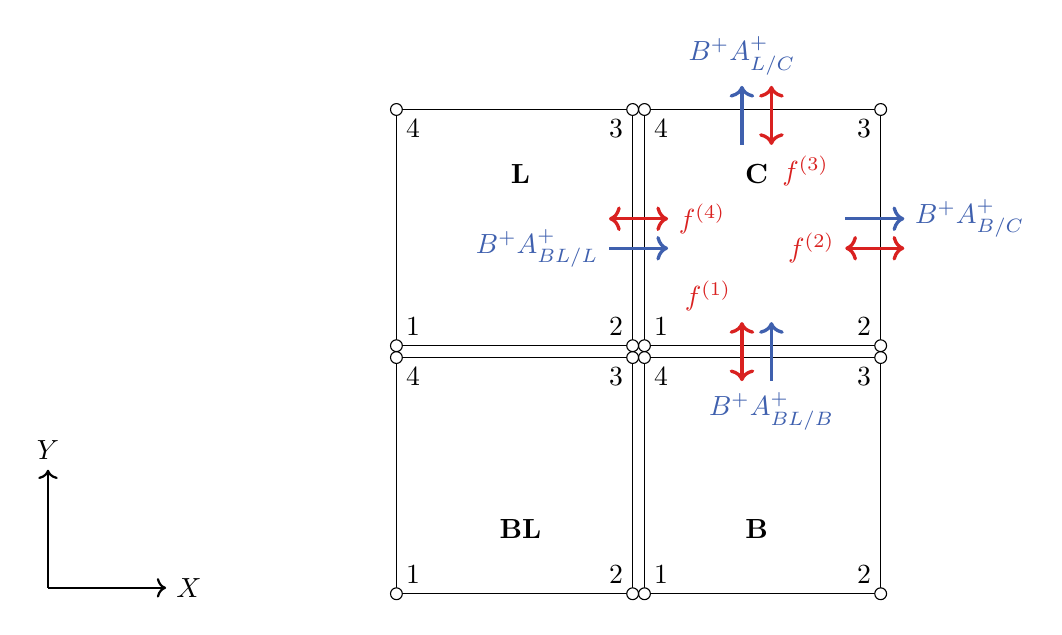
\begin{tikzpicture}[scale=1.5]
  \draw[thick,->] (-3,0.)-- (-2,0.) node[right] {$X$};
  \draw[thick,->] (-3,0.)-- (-3,1.) node[above] {$Y$};

  %% Cells
  \draw (0-0.05,0-0.05) rectangle (2.-0.05,2-0.05);
  \draw (0-0.05,2+0.05) rectangle (2.-0.05,4+0.05);
  \draw (2+0.05,0-0.05) rectangle (4.+0.05,2-0.05);
  \draw (2+0.05,2+0.05) rectangle (4.+0.05,4+0.05);
  %%%%%%%%%%%%%%%%%%%%%
  
  %% Nodes
  \fill[white] (0-0.05,0-0.05) circle (0.05);\fill[white] (2-0.05,2-0.05) circle (0.05);
  \fill[white] (0-0.05,2+0.05) circle (0.05);\fill[white] (2.-0.05,4+0.05) circle (0.05);
  \fill[white] (2+0.05,0-0.05) circle (0.05);\fill[white] (4.+0.05,2-0.05) circle (0.05);
  \fill[white] (2+0.05,2+0.05) circle (0.05);\fill[white] (4.+0.05,4+0.05) circle (0.05);
  \fill[white] (2-0.05,0-0.05) circle (0.05);\fill[white] (4.+0.05,0-0.05) circle (0.05);
  \fill[white] (0-0.05,2-0.05) circle (0.05);\fill[white] (2.+0.05,2-0.05) circle (0.05);
  \fill[white] (2-0.05,2+0.05) circle (0.05);\fill[white] (4.+0.05,2.+0.05) circle (0.05);
  \fill[white] (-0.05,4+0.05) circle (0.05);\fill[white] (2.+0.05,4+0.05) circle (0.05);

  \draw (0-0.05,0-0.05) circle (0.05) node[above right] {$1$};\draw (2-0.05,2-0.05) circle (0.05) node[below left] {$3$};
  \draw (0-0.05,2+0.05) circle (0.05) node[above right] {$1$};\draw (2.-0.05,4+0.05) circle (0.05) node[below left] {$3$};
  \draw (2+0.05,0-0.05) circle (0.05) node[above right] {$1$};\draw (4.+0.05,2-0.05) circle (0.05) node[below left] {$3$};
  \draw (2+0.05,2+0.05) circle (0.05) node[above right] {$1$};\draw (4.+0.05,4+0.05) circle (0.05) node[below left] {$3$};
  \draw (2-0.05,0-0.05) circle (0.05) node[above left] {$2$};\draw (4.+0.05,0-0.05) circle (0.05) node[above left] {$2$};
  \draw (0-0.05,2-0.05) circle (0.05) node[below right] {$4$};\draw (2.+0.05,2-0.05) circle (0.05) node[below right] {$4$};
  \draw (2-0.05,2+0.05) circle (0.05) node[above left] {$2$};\draw (4.+0.05,2.+0.05) circle (0.05) node[above left] {$2$};
  \draw (-0.05,4+0.05) circle (0.05) node[below right] {$4$};\draw (2.+0.05,4+0.05) circle (0.05) node[below right] {$4$};
  %%%%%%%%%%%%%%%%%%%%%%%

  %% Cells names
  \node at (3,3.5) {$\textbf{C}$};
  \node at (1,0.5) {$\textbf{BL}$};
  \node at (3,0.5) {$\textbf{B}$};
  \node at (1,3.5) {$\textbf{L}$};

  %% Transverse corrections
  \draw[->, very thick,Blue] (2.875,3.75) -- (2.875,4.25) node [above] {$B^+A^+_{L/C}$}; % Top
  \draw[->, very thick,Blue] (3.75,3.125) -- (4.25,3.125) node [right] {$B^+A^+_{B/C}$}; % Right
  \draw[<-, very thick,Blue] (3.125,2.25) -- (3.125,1.75) node [below] {$B^+A^+_{BL/B}$}; % Bottom
  \draw[<-, very thick,Blue] (2.25,2.875) -- (1.75,2.875) node [left] {$B^+A^+_{BL/L}$}; % Left

  %% Normal fluxes
  \draw[<->, very thick,Red] (3.125,3.75) node [below right] {$f^{(3)}$} -- (3.125,4.25) ; % Top
  \draw[<->, very thick,Red] (3.75,2.875) node [left] {$f^{(2)}$}-- (4.25,2.875) ; % Right
  \draw[<->, very thick,Red] (2.875,2.25) node [above left] {$f^{(1)}$}-- (2.875,1.75); % Bottom
  \draw[<->, very thick,Red] (2.25,3.125) node [right] {$f^{(4)}$} -- (1.75,3.125); % Left

  % %% Edges numbers
  % \node[above] at (1,-0.1) {$(1)$};
  % \node[left] at (2,1.) {$(2)$};
  % \node[below] at (1,1.95) {$(3)$};
  % \node[right] at (-0.1,1.) {$(4)$};
\end{tikzpicture}


%%% Local Variables:
%%% mode: latex
%%% TeX-master: "../../mainManuscript"
%%% End:

  \caption{Two-dimensional patch of cells of constant size $\Delta x \times \Delta x$.}\label{fig:2Dmesh}
\end{figure}
Figure \ref{fig:2Dmesh} shows transverse corrections in the cell $C$ based on fluctuations coming from Bottom ($B$), Left ($L$) and Bottom Left ($BL$) neighbor elements. The use of the numbering of interfaces and nodes adopted in figure \ref{fig:2Dmesh} allows the specialization of equation \eqref{eq:CTU-fluxes} to intercell fluxes of cell $C$:
\begin{align}
  & F_n^{(1)} = s_2 \frac{q_3^{B,k} + q_4^{B,k}}{2} - s_1 s_2 \frac{\Delta t}{2\Delta y}\(\frac{q_1^{B,k}+q_4^{B,k}}{2}-\frac{q_2^{BL,k}+q_3^{BL,k}}{2}\) \\
  & F_n^{(2)} = s_1 \frac{q_2^{C,k} + q_3^{C,k}}{2} - s_1 s_2 \frac{\Delta t}{2\Delta x}\(\frac{q_1^{C,k}+q_2^{C,k}}{2}-\frac{q_3^{B,k}+q_4^{B,k}}{2}\) \\
  & F_n^{(3)} = s_2 \frac{q_3^{C,k} + q_4^{C,k}}{2} - s_1 s_2 \frac{\Delta t}{2\Delta y}\(\frac{q_1^{C,k}+q_4^{C,k}}{2}-\frac{q_2^{L,k}+q_3^{L,k}}{2}\) \\
  & F_n^{(4)} = s_1 \frac{q_3^{L,k} + q_4^{L,k}}{2} - s_1 s_2 \frac{\Delta t}{2\Delta x}\(\frac{q_1^{L,k}+q_2^{L,k}}{2}-\frac{q_3^{BL,k}+q_4^{BL,k}}{2}\)
\end{align}
% where $q^{C,k}_i= \rho \bar{q}^{C,k}_i$ is the value at time step $k$ and node $i$ of cell $C$.
Denoting the number of particles in cell $C$ and the mass they carry by $N_p^C$ and $m^C$ respectively, the mass density reads $\rho = \frac{N_p^{C} m^C}{\Delta x \Delta y}$.
Thus, introduction of the particle fields projection yields the following expressions for interface fluxes:
\begin{align}
  & F_n^{(1)} = \sum_{J=1}^{N_p}\bar{Q}_J^k\frac{s_2 N^C_p m^C }{2\Delta x \Delta y} \[  \(\frac{S_{3J}^{B} }{\sum_L S_{3L}^{B}} + \frac{S_{4J}^{B}}{\sum_L S_{4L}^{B}}\) - s_1  \frac{\Delta t}{2\Delta y}\(\frac{S_{1J}^{B}}{\sum_L S_{1L}^B} + \frac{S_{4J}^{B}}{\sum_L S_{4L}^{B} }-\frac{S_{2J}^{BL}}{\sum_L S_{2L}^{BL}} - \frac{S_{3J}^{BL}}{\sum_L S_{3L}^{BL}}\) \]\\
  & F_n^{(2)} = \sum_{J=1}^{N_p} \bar{Q}_J^k\frac{s_1 N^C_p m^C }{2\Delta x \Delta y} \[  \(\frac{S_{2J}^{C}}{\sum_L S_{2L}^{C}} + \frac{S_{3J}^{C}}{\sum_L S_{3L}^{C}} \)- s_2 \frac{\Delta t}{2\Delta x}\(\frac{S_{1J}^{C}}{\sum_L S_{1L}^{C}} + \frac{S_{2J}^{C}}{\sum_L S_{2L}^{C}}-\frac{S_{3J}^{B}}{\sum_L S_{3L}^{B}} -\frac{S_{4J}^{B}}{\sum_L S_{4L}^{B}}\) \]\\
  & F_n^{(3)} =\sum_{J=1}^{N_p}\bar{Q}_J^k\frac{s_2 N^C_p m^C}{2\Delta x \Delta y} \[  \(\frac{S_{3J}^{C}}{\sum_L S_{3L}^{C}} + \frac{ S_{4J}^{C}}{\sum_L S_{4L}^{C}}\) - s_1  \frac{\Delta t}{2\Delta y}\( \frac{S_{1J}^{C}}{\sum_L S_{1L}^{C}} + \frac{S_{4J}^{C}}{\sum_L S_{4L}^{C}}-\frac{S_{2J}^{L}}{\sum_L S_{2L}^{L}} - \frac{S_{3J}^{L}}{\sum_L S_{3L}^{L}}\) \]\\
  & F_n^{(4)} = \sum_{J=1}^{N_p}\bar{Q}_J^k\frac{s_1 N^C_p m^C }{2\Delta x \Delta y}  \[  \(\frac{S_{3J}^{L}}{\sum_L S_{3L}^{L}} + \frac{ S_{4J}^{L}}{\sum_L S_{4L}^{L}}\) - s_2 \frac{\Delta t}{2\Delta x}\( \frac{S_{1J}^{L}}{\sum_L S_{1L}^{L}} + \frac{S_{2J}^{L}}{\sum_L S_{2L}^{L}}-\frac{S_{3J}^{BL}}{\sum_L S_{3L}^{BL}} - \frac{S_{4J}^{BL}}{\sum_L S_{4L}^{L}}\)\]
\end{align}
written for simplicity:
\begin{equation}
  \label{eq:interface_flux_mapped}
  F_n^{(i)}=\sum^{N_p}_J \bar{Q}_J^k \frac{s_n N^C_p m^C}{2\Delta x \Delta y}\[ \phi_J^{(i)} + \phi_J^{(i),T} \]
\end{equation}
In the latter expressions, $\phi^{(i)}$ is devoted to normal contributions while $\phi^{(i),T}$ stands for transverse corrections at interface $(i)$. Numerical fluxes considered above are based on normal vectors oriented in the direction of the stream (see figure \ref{fig:2Dmesh}). Nodal interface fluxes on the other hand, as defined in the semi-discrete system:
%Fluxes contribute to nodes through the boundary integrals of the discrete form:
\begin{equation}
  \hat{F}_i = \int_{l} S_i(\vect{x}) F_n  \: dl
\end{equation}
are based on the outgoing flux to an element so that $F_n^{(1)}$ and $F_n^{(4)}$ must be counted negatively. The integral for cell $C$ is then:
\begin{equation}
  \hat{F}_i =  -\int_{x^C_1}^{x_2^C} S_i(x,y^C_{1}) F_n^{(1)}  dx + \int_{y^C_2}^{y_3^C} S_i(x^C_{2},y) F_n^{(2)}  dy +\int_{x^C_2}^{x_3^C} S_i(x,y^C_{3}) F_n^{(3)}  dx -\int_{y^C_1}^{y_4^C} S_i(x^C_{1},y) F_n^{(4)}  dy 
\end{equation}
which can be computed analytically by using parent coordinates \eqref{eq:parentCoordinates}:
\begin{subequations}
  \begin{alignat}{4}
    &\hat{F}_1 = -&\frac{1}{2}\[\Delta x F_n^{(1)} + \Delta y F_n^{(4)}\] \quad;\quad &\hat{F}_2 = -&\frac{1}{2}\[\Delta x F_n^{(1)} - \Delta y F_n^{(2)}\]\\
    &\hat{F}_3 =  &\frac{1}{2}\[\Delta x F_n^{(3)} + \Delta y F_n^{(2)}\] \quad;\quad &\hat{F}_4 = &\frac{1}{2}\[\Delta x F_n^{(3)} - \Delta y F_n^{(4)}\]
  \end{alignat}
\end{subequations}
A condensed way of writing those fluxes is adopted by means of the middle point of edge $(j)$ with coordinates $\vect{x}^{(j)}_{1/2}$, at which the shape functions are:
\begin{equation*}
  S_i(\vect{x}^{(j)}_{1/2}) =
  \left\lbrace
  \begin{aligned}
    & \frac{1}{2} \quad \text{if node i belongs to edge (j)} \\
    & 0 \quad \text{otherwise.}
  \end{aligned}
  \right.
\end{equation*}
In addition, components of the outward normal vector to edges $n^{(i)}_x$ and $n^{(i)}_y$ allow to take into account different signs of intercell fluxes in the Cartesian grid. One thus writes:
\begin{equation}
  \hat{F}_i= \frac{1}{2}\sum_{j=1}^{\text{Nedges}} 2S_{i}(\vect{x}^{(j)}_{1/2})\(\Delta y n^{(j)}_x + \Delta x n^{(j)}_y\) F_n^{(j)}
\end{equation}
which, combined to equation \eqref{eq:interface_flux_mapped} leads to:
\begin{equation}
  \hat{F}^k_i= \sum^{N_p}_J \bar{Q}_J^k \sum_{j=1}^{\text{Nedges}} S_{i}(\vect{x}^{(j)}_{1/2})\(s_1\Delta y n^{(j)}_x + s_2\Delta x n^{(j)}_y\)  \frac{ N^C_p m^C}{2\Delta x\Delta y}\[ \phi_J^{(i)} + \phi_J^{(i),T} \]
\end{equation}
These terms are divided by the lumped mass matrix in the discrete form:
\begin{equation}
  \label{eq:nodal_fluxes}
  \frac{\hat{F}^k_i}{M_i^L}=\sum_J \frac{\bar{Q}_J^k}{\sum_K S_{iK}}   \sum_{j=1}^{\text{Nedges}}\frac{1}{2} S_{i}(\vect{x}^{(j)}_{1/2}) N^C_p m^C \(s_1\frac{n^{(j)}_x}{\Delta x}  + s_2\frac{n^{(j)}_y}{\Delta y} \) \[\phi_J^{(j)} + \phi_J^{(j),T}\] 
\end{equation}

At last, gathering the mapping of updated nodal quantities to the particle \eqref{eq:2D_updatedMP}, expressions of volume fluxes \eqref{eq:2Dvolume_fluxes} and intercell ones \eqref{eq:nodal_fluxes}, the updated value at material point $I$ contained in cell $C$ reads:
\begin{equation}
  \label{eq:2Dscheme_equation}
  \begin{split}
    \bar{Q}_I^{k+1}=  \sum_{L=1}^{N_p}\bar{Q}_L^k\sum_{i=1}^{4E}\frac{S_{iI}}{\sum_K S_{iK}}  \left\lbrace \vphantom{\sum_{j=1}^{\text{edges}} } \right.& S_{iL} +  2  \sum_{j=1}^{4E} \frac{ S_{jL}}{\sum_K S_{jK}}\sum_{J=1}^{N_p}S_{jJ}\[ s_1\frac{\Delta t}{\Delta x}\partial_\xi S_{iJ}  + s_2\frac{\Delta t}{\Delta y} \partial_\eta S_{iJ} \] \\ - & \frac{1}{2}\left.\sum_{p=1}^{\text{edges}} S_{i}(\vect{x}^{(p)}_{1/2}) N_p^C \(s_1\frac{\Delta t}{\Delta x}n^{(j)}_x  + s_2\frac{\Delta t}{\Delta y}n^{(j)}_y \)\[\phi_L^{(p)} + \phi_L^{(p),T}\] \right\rbrace
  \end{split}
\end{equation}
Recall that transverse contributions $\phi_L^{(p),T}$ depend on $\Delta t$, thus providing second-order corrections in the two-dimensional scheme equation \eqref{eq:2Dscheme_equation}, that can also be rewritten as:
\begin{equation}
  \label{eq:2Dscheme_D_alphabeta}
  \bar{Q}_I^{k+1}= \sum_{L=1}^{N_p}\bar{Q}_L^k H_{IL}
\end{equation}

\subsection{The von Neumann linear stability analysis}
Analogously to the one-dimensional case, the solution at a material point can be expanded into a discrete Fourier basis over the domain $\[-l,l\]\times\[-h,h\]$. We consider here a structured distribution of particles made of $N_p=N_p^x\times N_p^y$ material points so that one can denote the solution at particles by $\bar{Q}_{IL}$, where $I$ and $L$ are the row and column of material points indices. For one arbitrary Fourier mode, one has \cite{Leveque}:
\begin{equation}
\bar{Q}^{k}_{I L} = A_{jq}^k e^{i (I \lambda_j\Delta y + L \lambda_q\Delta x)}
\end{equation}
where $i=\sqrt{-1}$, and $\lambda_j$ and $\lambda_q$ are wave numbers in directions $x$ and $y$ respectively.
Then, the amplification factor reads:
\begin{equation}
\frac{A_{jq}^{k+1}}{A_{jq}^k} =  \sum_{K=1}^{N_p^y}\sum_{J=1}^{N_p^x} e^{i ([I-K]\lambda_j\Delta y + [L-J]\lambda_q\Delta x)}H_{IL,KJ}
\end{equation}
The requirement that the absolute value of the amplification factor is lower than or equal to one leads to the following stability condition:
\begin{equation}
\abs{\frac{A_{jq}^{k+1}}{A_{jq}^k}} = \abs{\sum_{K=1}^{N_p^y}\sum_{J=1}^{N_p^x} e^{i ([I-K]\lambda_j\Delta y + [L-J]\lambda_q\Delta x)}H_{IL,KJ}} \leq 1 \Leftrightarrow  \sum_{K=1}^{N_p^y}\sum_{J=1}^{N_p^x} \abs{H_{IL,KJ}} \leq 1
\end{equation}
or more simply:
\begin{equation}
\label{eq:2D_stability}
\sum_{L=1}^{N_p} \abs{H_{IL}} \leq 1 \quad \forall I=1,...,N_p
\end{equation}


\subsection{Evaluation of the CFL number for particular space discretizations}
Again the study of stability conditions for general discretizations is complicated given the scheme equation \eqref{eq:2Dscheme_equation}.
Nevertheless, it can first be noticed that the single particle-per-cell discretization leads to a piece-wise constant reconstruction of the field on the computational grid after the projection from material points to nodes whatever their locations in cells.
Therefore, the first-order upwind method is once again retrieved.
This method is known to be characterized by \cite{Leveque}:
\begin{subequations}
  \begin{alignat}{2}
    \label{eq:2DCFL_DCU}
    & \abs{s_1}\frac{\Delta t}{\Delta x} + \abs{s_2} \frac{\Delta t}{\Delta y} \leq 1 \qquad &\text{for DCU} \\
    \label{eq:2DCFL_CTU}
    & \max \( \abs{s_1} \frac{\Delta t}{\Delta x}  , \abs{s_2} \frac{\Delta t}{\Delta y}\) \leq 1 \qquad &\text{for CTU}
  \end{alignat}
\end{subequations}


From now on, it is assumed that $s_1\geq s_2 >0$ and regular cells $\Delta x = \Delta y$ are considered.
In that case, the critical time steps resulting from conditions \eqref{eq:2DCFL_DCU} and \eqref{eq:2DCFL_CTU} read:
\begin{equation}
  \Delta t \leq \frac{\Delta x}{s_1+s_2} \quad \text{for DCU} \quad;\quad \Delta t \leq \frac{\Delta x}{s_1} \quad \text{for CTU}
\end{equation}
In terms of Courant number, the previous conditions are:
\begin{subequations}
  \begin{alignat}{2}
    \label{eq:2D_CFL_DCU}
    & s_1\frac{\Delta t}{\Delta x} \leq \frac{s_1}{s_1+s_2} \qquad &\text{for DCU} \\
    \label{eq:2D_CFL_CTU}
    & s_1\frac{\Delta t}{\Delta x} \leq 1 \qquad &\text{for CTU}
  \end{alignat}
\end{subequations}
Hence, the CFL number can be set at one by using the CTU regardless of the speeds values.
Conversely, the maximal Courant number governing the DCU tends to one if and only if $s_1 \gg s_2$.


Configurations involving more particles in the computational grid cells are now studied numerically by assuming the same material points distribution in every elements.
%Furthermore, we consider only regular cells $\Delta y = \Delta x$ and wave speeds satisfying $a\geq b >0$, so that Courant number reads $a\Delta t/\Delta x$.
Since the coefficients $H_{I J}$ depend on both horizontal and vertical wave speeds, the scheme equation \eqref{eq:2Dscheme_D_alphabeta} can be written as a function of the CFL number by means of the speed ratio  $s_1/s_2$.
Hence, the maximal Courant number satisfying the stability condition \eqref{eq:2D_stability} also depends on the speed ratio.
Evolutions of the CFL numbers corresponding to several distributions of particles in a two-dimensional grid are gathered in tables \ref{tab:2DCFL_comparison_2ppc}, \ref{tab:2DCFL_comparison_4ppc} and \ref{tab:2DCFL_comparison_9ppc} for the DGMPM scheme using DCU and CTU methods.
The first column of these tables shows the positions of material points inside cells for discretizations based on two, four or nine particles per element respectively. 

%% 2ppc
The space discretization leading to two particles lying in every cells of the mesh is such that within an element, the two material points are both either on the horizontal axis or on the vertical axis of the cell.
The aforementioned cases respectively correspond to the results reported in first and second rows of table \ref{tab:2DCFL_comparison_2ppc}.
Two situations are then to be distinguished:
\begin{itemize}
\item Material points are regularly-spaced within the grid and placed symmetrically two-by-two with respect to cells centers.
  Those distributions are drawn in the first column of table \ref{tab:2DCFL_comparison_2ppc} by using blue plus signs to represent particles.
\item Material points still satisfy symmetry in cells, but are no longer regularly-spaced in the mesh.
  In that case, particles are drawn with red crosses.
\end{itemize}
\begin{table}[h!]
  \centering
  \input{tabular/2DCFL_comparison_2ppc}
  \caption{Values of critical Courant number $s_1\frac{\Delta t}{\Delta x}$ for two-dimensional DGMPM scheme using either DCU or CTU with respect to the locations of the two material points lying in every cells, as a function of the speeds ratio $s_1/s_2$.}
  \label{tab:2DCFL_comparison_2ppc}
\end{table}
First, the results of table \ref{tab:2DCFL_comparison_2ppc} show that the CFL number exhibits a non-linear dependence on the speed ratio $s_1/s_2$, which asymptotically approach some value depending on the particles distribution.
The configuration in which the particles are regularly spaced in the grid is of particular interest.
Indeed, this discretization is equivalent to the vertical repetition of the natural configuration for two particles per cell studied in section \ref{sec:1d_stab}.
As a result, the one-dimensional result for Euler discretization $CFL \approx 0.43$ should be recovered for $s_1 \gg s_2$.
This value is depicted with black dashed lines in the plots of first row in table \ref{tab:2DCFL_comparison_2ppc}.
It is thus seen that the one-dimensional value of the Courant number corresponds to the asymptotic limit for two-dimensional problems as $s_1/s_2 \rightarrow \infty$.
% In particular, the configuration drawn in blue plus signs in the first row is equivalent, for $s_1 \gg s_2$, to the one-dimensional natural configuration for two particles per cell studied in section \ref{sec:1d_stab}.
% As a result, the CFL number tends to the value $0.43$ determined in one space dimension as $s_1/s_2 \rightarrow \infty$, which is depicted with the black dashed lines in the CFL curves.

Next, the spacing between particles is reduced while keeping the symmetry with respect to cells centers.
It is then seen that, as for one-dimensional case, the critical Courant number increases for both DCU and CTU approaches.
%Second, we see that a reduction of spacing between particles ensuring symmetry between them with respect to cells centers, as for one-dimensional case, yields an increase in the critical Courant number for both DCU and CTU approaches. 
Third, whether particles lie on the horizontal axis or the vertical axis of cells has a great influence on the critical Courant number one can expect.
Hence, the configurations of the second row of table \ref{tab:2DCFL_comparison_2ppc} yield higher CFL numbers for given speed ratios.
It then appears that in order to improve the stability of the scheme, one must use a lower number of material points in the direction of the dominating wave speed than in the perpendicular one.
For a Cartesian distribution of particles $N_p^x \times N_p^y$ this corresponds to $N_p^y > N_p^x$ if $s_1>s_2$, and $N_p^x > N_p^y$ if $s_2>s_1$.
At last, it is worth noticing that the improvement brought by the CTU is much less significant than in the case of one single particle-per-cell discretization for which the Courant number can be set to one according to equations \eqref{eq:2D_CFL_DCU} and \eqref{eq:2D_CFL_CTU}.

%% 4ppc
\begin{table}[h!]
  \centering
  \begin{tabular}[ht]{M{2.5cm}M{5.cm}M{5.cm}N}
  %\setlength\extrarowheight{2.5pt}
  \hline
  Particles in cells & \multicolumn{2}{c}{Critical Courant number $\frac{a\Delta t}{\Delta X}(a/b)$}  & \\[0.5cm]
   &  DCU & CTU & \\
%   & & \multicolumn{2}{c}{$a/b=1$} & \multicolumn{2}{c}{$a/b=10$} & \multicolumn{2}{c}{$a/b=1$} & \multicolumn{2}{c}{$a/b=10$}\\
   % Particles & Position of particles in cell $c$ &  \multicolumn{2}{c}{DCU} & \multicolumn{2}{c}{DCU} \\
  \hline
  \hline
  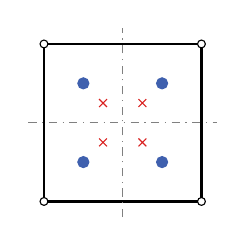
\begin{tikzpicture}[scale=1.]
    \draw[black,thick] (-1.,-1.) rectangle (1.,1.);
    \draw[black!50,dashdotted] (-1.2,0.) -- (1.2,0.0);\draw[black!50,dashdotted] (.0,-1.2) -- (0.,1.2);
    %% nodes
    \fill[white] (-1,-1) circle (0.05);\draw (-1,-1) circle (0.05);
    \fill[white] (1.,-1) circle (0.05);\draw (1,-1) circle (0.05);
    \fill[white] (1,1) circle (0.05);\draw (1,1) circle (0.05);
    \fill[white] (-1.,1) circle (0.05);\draw (-1,1) circle (0.05);
    %% particles
    \draw[Blue,mark=*] plot coordinates {(-0.5,-0.5)};
    \draw[Blue,mark=*] plot coordinates {(0.5,0.5)};
    \draw[Blue,mark=*] plot coordinates {(-0.5,0.5)};
    \draw[Blue,mark=*] plot coordinates {(0.5,-0.5)};
    %\draw[Blue,|-|] (0.5,-0.5) -- (0.5,0.5) node [midway,right] {\scriptsize $\frac{\Delta X}{2}$};
    \draw[Red,mark=x] plot coordinates {(-0.25,-0.25)};
    \draw[Red,mark=x] plot coordinates {(0.25,0.25)};
    \draw[Red,mark=x] plot coordinates {(-0.25,0.25)};
    \draw[Red,mark=x] plot coordinates {(0.25,-0.25)};
    %\draw[Red,|-|] (-0.25,-0.25) -- (-0.25,0.25) node [midway,left] {\scriptsize $\frac{\Delta X}{4}$};
  \end{tikzpicture} & 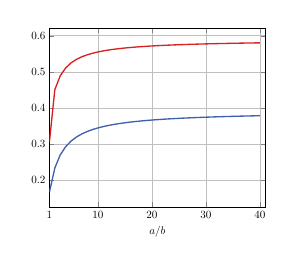
\begin{tikzpicture}[scale=0.4]
\begin{axis}[xlabel=$a/b$,ymajorgrids=true,xmajorgrids=true,xmin=1,xmax=41,xtick={1,10,20,30,40}]
%%%%%%%%%%% NATURAL CONFIGURATION
\addplot[Blue,very thick] coordinates {(1.0,0.166666666667) (2.0,0.233766233766) (3.0,0.27) (4.0,0.292682926829) (5.0,0.308219178082) (6.0,0.319526627219) (7.0,0.328125) (8.0,0.33488372093) (9.0,0.340336134454) (10.0,0.344827586207) (11.0,0.348591549296) (12.0,0.351791530945) (13.0,0.354545454545) (14.0,0.356940509915) (15.0,0.359042553191) (16.0,0.360902255639) (17.0,0.362559241706) (18.0,0.36404494382) (19.0,0.365384615385) (20.0,0.366598778004) (21.0,0.367704280156) (22.0,0.368715083799) (23.0,0.369642857143) (24.0,0.370497427101) (25.0,0.371287128713) (26.0,0.372019077901) (27.0,0.372699386503) (28.0,0.373333333333) (29.0,0.373925501433) (30.0,0.374479889043) (31.0,0.375) (32.0,0.375488917862) (33.0,0.375949367089) (34.0,0.376383763838) (35.0,0.376794258373) (36.0,0.377182770664) (37.0,0.377551020408) (38.0,0.377900552486) (39.0,0.378232758621) (40.0,0.378548895899) };
%%%%%%%%%%% MODIFIED CONFIGURATION
\addplot[Red,very thick] coordinates {(1.0,0.30612244898) (2.0,0.450574712644) (3.0,0.488913525499) (4.0,0.510638297872) (5.0,0.524625267666) (6.0,0.534383520145) (7.0,0.541578947368) (8.0,0.547103977669) (9.0,0.551479783243) (10.0,0.555031149707) (11.0,0.557971014493) (12.0,0.560444797458) (13.0,0.562555195761) (14.0,0.564376799671) (15.0,0.565965092402) (16.0,0.567362199976) (17.0,0.568600682594) (18.0,0.569706103994) (19.0,0.570698814875) (20.0,0.571595217265) (21.0,0.572408677916) (22.0,0.57315019938) (23.0,0.57382892057) (24.0,0.574452495319) (25.0,0.575027382256) (26.0,0.575559069347) (27.0,0.576052249637) (28.0,0.576510960151) (29.0,0.576938692651) (30.0,0.577338482686) (31.0,0.577712981744) (32.0,0.578064516129) (33.0,0.578395135328) (34.0,0.578706652) (35.0,0.579000675219) (36.0,0.579278638279) (37.0,0.579541822056) (38.0,0.579791374747) (39.0,0.580028328612) (40.0,0.58025361425) };
\end{axis}
\end{tikzpicture}
%%% Local Variables:
%%% mode: latex
%%% TeX-master: "../../mainManuscript"
%%% End:
 & 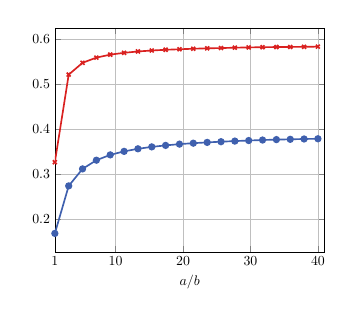
\begin{tikzpicture}[scale=0.5]
\begin{axis}[xlabel=$a/b$,ymajorgrids=true,xmajorgrids=true,xmin=1,xmax=41,xtick={1,10,20,30,40}]
%%%%%%%%%%% NATURAL CONFIGURATION
\addplot[Blue,mark=*,very thick] coordinates {(1.0,0.168781687817) (3.05263157895,0.274434323291) (5.10526315789,0.312241017147) (7.15789473684,0.331556999781) (9.21052631579,0.343371854771) (11.2631578947,0.351188775046) (13.3157894737,0.356866726562) (15.3684210526,0.361161506352) (17.4210526316,0.364452065573) (19.4736842105,0.367277356984) (21.5263157895,0.3693952729) (23.5789473684,0.371136342942) (25.6315789474,0.372686884764) (27.6842105263,0.374017424385) (29.7368421053,0.375282700195) (31.7894736842,0.376391132332) (33.8421052632,0.377343247117) (35.8947368421,0.377975358701) (37.9473684211,0.378718524027) (40.0,0.379203792038) };
%%%%%%%%%%% MODIFIED CONFIGURATION
\addplot[Red,mark=x,very thick] coordinates {(1.0,0.327083270833) (3.05263157895,0.521791533705) (5.10526315789,0.548055480555) (7.15789473684,0.559609806624) (9.21052631579,0.566176714399) (11.2631578947,0.570259386804) (13.3157894737,0.573250469347) (15.3684210526,0.575399438205) (17.4210526316,0.576991033068) (19.4736842105,0.578179466005) (21.5263157895,0.579278950684) (23.5789473684,0.580283697574) (25.6315789474,0.580817387121) (27.6842105263,0.581651079669) (29.7368421053,0.582253190953) (31.7894736842,0.5827068797) (33.8421052632,0.583105304737) (35.8947368421,0.583295306637) (37.9473684211,0.583636362679) (40.0,0.584005840058) };
\end{axis}
\end{tikzpicture}
%%% Local Variables:
%%% mode: latex
%%% TeX-master: "../../mainManuscript"
%%% End:
& \\ [3.25cm]
  %%%%%%%%%%%%%%%%%%%%%%%%%%%%%%%%%%%%%%%
  %%%%%%%%%%%%%%%%%%%%%%%%%%%%%%%%%%%%%%% 
  \hline % Shifted left // Shifted right
  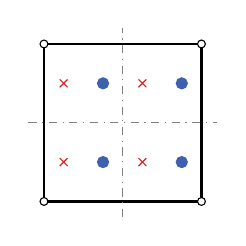
\begin{tikzpicture}[scale=1.]
    \draw[black,thick] (-1.,-1.) rectangle (1.,1.);
    \draw[black!50,dashdotted] (-1.2,0.) -- (1.2,0.0);\draw[black!50,dashdotted] (.0,-1.2) -- (0.,1.2);
    %% nodes
    \fill[white] (-1,-1) circle (0.05);\draw (-1,-1) circle (0.05);
    \fill[white] (1.,-1) circle (0.05);\draw (1,-1) circle (0.05);
    \fill[white] (1,1) circle (0.05);\draw (1,1) circle (0.05);
    \fill[white] (-1.,1) circle (0.05);\draw (-1,1) circle (0.05);
    %% particles
    \draw[Blue,mark=*] plot coordinates {(-0.5+0.25,-0.5)};
    \draw[Blue,mark=*] plot coordinates {(0.5+0.25,0.5)};
    \draw[Blue,mark=*] plot coordinates {(-0.5+0.25,0.5)};
    \draw[Blue,mark=*] plot coordinates {(0.5+0.25,-0.5)};
    \draw[Red,mark=x] plot coordinates {(-0.5-0.25,-0.5)};
    \draw[Red,mark=x] plot coordinates {(0.5-0.25,0.5)};
    \draw[Red,mark=x] plot coordinates {(-0.5-0.25,0.5)};
    \draw[Red,mark=x] plot coordinates {(0.5-0.25,-0.5)};
  \end{tikzpicture}  & 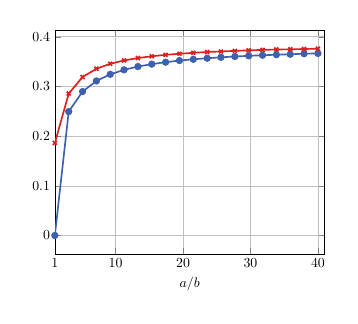
\begin{tikzpicture}[scale=0.5]
\begin{axis}[xlabel=$a/b$,ymajorgrids=true,xmajorgrids=true,xmin=1,xmax=41,xtick={1,10,20,30,40}]
%%%%%%%%%%% NATURAL CONFIGURATION
\addplot[Blue,mark=*,very thick] coordinates {(1.0,1.0000100001e-05) (3.05263157895,0.249310914162) (5.10526315789,0.28957342205) (7.15789473684,0.311013636452) (9.21052631579,0.324305874638) (11.2631578947,0.333392807612) (13.3157894737,0.339955504818) (15.3684210526,0.344870817129) (17.4210526316,0.348772961414) (19.4736842105,0.352087731404) (21.5263157895,0.354541966472) (23.5789473684,0.356753041215) (25.6315789474,0.358589375367) (27.6842105263,0.360175180699) (29.7368421053,0.361603616036) (31.7894736842,0.362721521952) (33.8421052632,0.363806269642) (35.8947368421,0.364694173258) (37.9473684211,0.365816289742) (40.0,0.366403664037) };
%%%%%%%%%%% MODIFIED CONFIGURATION
\addplot[Red,mark=x,very thick] coordinates {(1.0,0.186161861619) (3.05263157895,0.285515486734) (5.10526315789,0.318877925621) (7.15789473684,0.335565460918) (9.21052631579,0.345582403192) (11.2631578947,0.352315102098) (13.3157894737,0.357133045015) (15.3684210526,0.36070044911) (17.4210526316,0.363581004231) (19.4736842105,0.365719446668) (21.5263157895,0.367673150416) (23.5789473684,0.36925000829) (25.6315789474,0.37038001959) (27.6842105263,0.371525820521) (29.7368421053,0.372606357643) (31.7894736842,0.37353005109) (33.8421052632,0.374297427185) (35.8947368421,0.37474480008) (37.9473684211,0.375303226716) (40.0,0.376003760038) };
\end{axis}
\end{tikzpicture}
%%% Local Variables:
%%% mode: latex
%%% TeX-master: "../../mainManuscript"
%%% End:
 &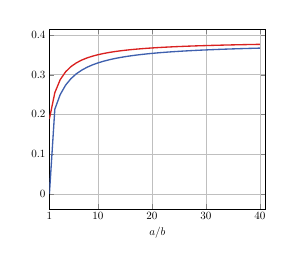
\begin{tikzpicture}[scale=0.4]
\begin{axis}[xlabel=$a/b$,ymajorgrids=true,xmajorgrids=true,xmin=1,xmax=41,xtick={1,10,20,30,40}]
%%%%%%%%%%% NATURAL CONFIGURATION
\addplot[Blue,very thick] coordinates {(1.0,-1.59364188514e-12) (2.0,0.212857320897) (3.0,0.249893924351) (4.0,0.27360416432) (5.0,0.290070593852) (6.0,0.30216822431) (7.0,0.311430129824) (8.0,0.318747857117) (9.0,0.324674954147) (10.0,0.329573175966) (11.0,0.333688883167) (12.0,0.337195633388) (13.0,0.340219213023) (14.0,0.342853009248) (15.0,0.345167807082) (16.0,0.347218235209) (17.0,0.349047125479) (18.0,0.350688533417) (19.0,0.352169876071) (20.0,0.3535134741) (21.0,0.354737683146) (22.0,0.355857736689) (23.0,0.356886382692) (24.0,0.357834370589) (25.0,0.358710828109) (26.0,0.359523555947) (27.0,0.360279260443) (28.0,0.360983738964) (29.0,0.361642028851) (30.0,0.362258527996) (31.0,0.362837093184) (32.0,0.36338112082) (33.0,0.363893613627) (34.0,0.364377236081) (35.0,0.364834360724) (36.0,0.365267107082) (37.0,0.365677374516) (38.0,0.36606687008) (39.0,0.366437132262) (40.0,0.366789551283) };
%%%%%%%%%%% MODIFIED CONFIGURATION
\addplot[Red,very thick] coordinates {(1.0,0.18887015067) (2.0,0.254459520239) (3.0,0.287403904864) (4.0,0.307169534548) (5.0,0.320334758075) (6.0,0.329729082668) (7.0,0.336768311765) (8.0,0.342238808871) (9.0,0.346612107914) (10.0,0.350188061313) (11.0,0.353166425063) (12.0,0.355685394958) (13.0,0.357843617559) (14.0,0.359713389803) (15.0,0.361348904135) (16.0,0.362791580609) (17.0,0.364073619671) (18.0,0.36522043174) (19.0,0.366252337065) (20.0,0.367185779335) (21.0,0.368034207917) (22.0,0.368808729666) (23.0,0.369518597597) (24.0,0.370171582133) (25.0,0.370774256583) (26.0,0.371332219112) (27.0,0.371850267081) (28.0,0.372332535292) (29.0,0.372782606539) (30.0,0.373203600747) (31.0,0.373598247379) (32.0,0.373968944663) (33.0,0.374317808349) (34.0,0.374646712123) (35.0,0.374957321245) (36.0,0.375251120754) (37.0,0.375529439201) (38.0,0.375793468735) (39.0,0.376044282167) (40.0,0.376282847537) };
\end{axis}
\end{tikzpicture}
%%% Local Variables:
%%% mode: latex
%%% TeX-master: "../../mainManuscript"
%%% End:
& \\ [3.25cm]
  %%%%%%%%%%%%%%%%%%%%%%%%%%%%%%%%%%%%%
  %%%%%%%%%%%%%%%%%%%%%%%%%%%%%%%%%%%%%
  \hline % Shifted above // Shifted below
  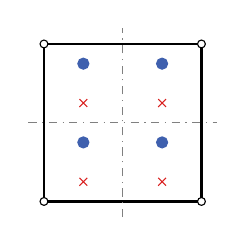
\begin{tikzpicture}[scale=1.]
    \draw[black,thick] (-1.,-1.) rectangle (1.,1.);
    \draw[black!50,dashdotted] (-1.2,0.) -- (1.2,0.0);\draw[black!50,dashdotted] (.0,-1.2) -- (0.,1.2);
    %% nodes
    \fill[white] (-1,-1) circle (0.05);\draw (-1,-1) circle (0.05);
    \fill[white] (1.,-1) circle (0.05);\draw (1,-1) circle (0.05);
    \fill[white] (1,1) circle (0.05);\draw (1,1) circle (0.05);
    \fill[white] (-1.,1) circle (0.05);\draw (-1,1) circle (0.05);
    %% particles
    \draw[Blue,mark=*] plot coordinates {(-0.5,-0.5+0.25)};
    \draw[Blue,mark=*] plot coordinates {(0.5,0.5+0.25)};
    \draw[Blue,mark=*] plot coordinates {(-0.5,0.5+0.25)};
    \draw[Blue,mark=*] plot coordinates {(0.5,-0.5+0.25)};
    \draw[Red,mark=x] plot coordinates {(-0.5,-0.5-0.25)};
    \draw[Red,mark=x] plot coordinates {(0.5,0.5-0.25)};
    \draw[Red,mark=x] plot coordinates {(-0.5,0.5-0.25)};
    \draw[Red,mark=x] plot coordinates {(0.5,-0.5-0.25)};
  \end{tikzpicture}& 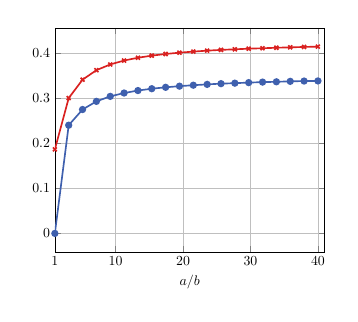
\begin{tikzpicture}[scale=0.5]
\begin{axis}[xlabel=$a/b$,ymajorgrids=true,xmajorgrids=true,xmin=1,xmax=41,xtick={1,10,20,30,40}]
%%%%%%%%%%% NATURAL CONFIGURATION
\addplot[Blue,mark=*,very thick] coordinates {(1.0,1.0000100001e-05) (3.05263157895,0.239878188256) (5.10526315789,0.274614851412) (7.15789473684,0.292689242682) (9.21052631579,0.303766195557) (11.2631578947,0.311204164673) (13.3157894737,0.316652640211) (15.3684210526,0.32074215479) (17.4210526316,0.323860607027) (19.4736842105,0.326382211191) (21.5263157895,0.328494863896) (23.5789473684,0.330344356075) (25.6315789474,0.331932266691) (27.6842105263,0.333044383075) (29.7368421053,0.334245447718) (31.7894736842,0.335382301191) (33.8421052632,0.336055465818) (35.8947368421,0.337054949497) (37.9473684211,0.337734956297) (40.0,0.338003380034) };
%%%%%%%%%%% MODIFIED CONFIGURATION
\addplot[Red,mark=x,very thick] coordinates {(1.0,0.186161861619) (3.05263157895,0.299954578493) (5.10526315789,0.340728670445) (7.15789473684,0.361763617636) (9.21052631579,0.374503745037) (11.2631578947,0.383176463344) (13.3157894737,0.389357577786) (15.3684210526,0.394050256292) (17.4210526316,0.397726608845) (19.4736842105,0.400577689987) (21.5263157895,0.402976661346) (23.5789473684,0.405090366693) (25.6315789474,0.406777225667) (27.6842105263,0.408069343851) (29.7368421053,0.409480410594) (31.7894736842,0.410406209325) (33.8421052632,0.411524115241) (35.8947368421,0.412434650662) (37.9473684211,0.413250974615) (40.0,0.414004140041) };
\end{axis}
\end{tikzpicture}
%%% Local Variables:
%%% mode: latex
%%% TeX-master: "../../mainManuscript"
%%% End:
 &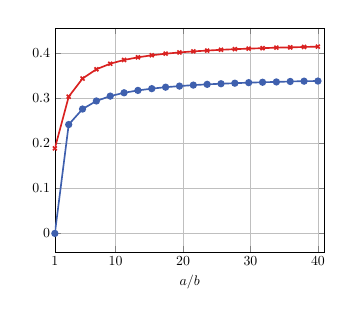
\begin{tikzpicture}[scale=0.5]
\begin{axis}[xlabel=$a/b$,ymajorgrids=true,xmajorgrids=true,xmin=1,xmax=41,xtick={1,10,20,30,40}]
%%%%%%%%%%% NATURAL CONFIGURATION
\addplot[Blue,mark=*,very thick] coordinates {(1.0,1.0000100001e-05) (3.05263157895,0.241770838761) (5.10526315789,0.276248551959) (7.15789473684,0.294120835945) (9.21052631579,0.304963575952) (11.2631578947,0.312330491726) (13.3157894737,0.317584754795) (15.3684210526,0.321510583527) (17.4210526316,0.324731668369) (19.4736842105,0.327161166349) (21.5263157895,0.329355925138) (23.5789473684,0.33105173157) (25.6315789474,0.332444903396) (27.6842105263,0.333598072823) (29.7368421053,0.334840190507) (31.7894736842,0.335700199107) (33.8421052632,0.336393890255) (35.8947368421,0.337413900455) (37.9473684211,0.338114433776) (40.0,0.338403384034) };
%%%%%%%%%%% MODIFIED CONFIGURATION
\addplot[Red,mark=x,very thick] coordinates {(1.0,0.188871888719) (3.05263157895,0.303648299641) (5.10526315789,0.343945018398) (7.15789473684,0.364483644836) (9.21052631579,0.376898505827) (11.2631578947,0.385203852039) (13.3157894737,0.391088647729) (15.3684210526,0.395587113766) (17.4210526316,0.399120306993) (19.4736842105,0.401940861514) (21.5263157895,0.404268253209) (23.5789473684,0.40603353402) (25.6315789474,0.407802499078) (27.6842105263,0.409176723346) (29.7368421053,0.410372524778) (31.7894736842,0.411359903073) (33.8421052632,0.412539388552) (35.8947368421,0.413152552578) (37.9473684211,0.414009929573) (40.0,0.414804148041) };
\end{axis}
\end{tikzpicture}
%%% Local Variables:
%%% mode: latex
%%% TeX-master: "../../mainManuscript"
%%% End:
& \\ [3.25cm]
  %\begin{minipage}{0.85\textwidth}\lipsum[1]\end{minipage}
  \hline
\end{tabular}

%%% Local Variables: 
%%% mode: latex
%%% TeX-master: "../../mainManuscript"
%%% End:
  \caption{Values of critical Courant number $s_1\frac{\Delta t}{\Delta x}$ for two-dimensional DGMPM scheme using either DCU or CTU with respect to the material points distribution, as a function of the speeds ratio $s_1/s_2$.}
  \label{tab:2DCFL_comparison_4ppc}
\end{table}
We now move on to cases for which grid cells each contains four material points, by considering a square shaped distribution of particles in every elements. %which centers coincide with cells centroids.
This square distribution is such that the particles are initially regularly spaced in horizontal and vertical directions, and is deformed so that the following situations occur:
\begin{itemize}
\item the particles are displaced while keeping the center of the square of material points on the cells centroids.
  Three configurations are then depicted in the first row of table \ref{tab:2DCFL_comparison_4ppc}.
\item the square of particles is translated horizontally without distortion as depicted in the second row of the table.
\item the square of particles is translated vertically without distortion (third row of the table).
\end{itemize}

%In the first row of table \ref{tab:2DCFL_comparison_4ppc}, the particles are displaced while keeping the center of the square of material points on the cells centroids.
%On the other hand, the second and third rows of the table investigate of a simple translation of the square pattern in the elements without distortion.  
% This pattern can be contracted or simply translated without change of shape as depicted in the first column of table \ref{tab:2DCFL_comparison_4ppc}.
%Several configurations are gathered in each row of the table and are distinguished by using different colors and markers.

First, we see in the first row of table \ref{tab:2DCFL_comparison_4ppc} that the contraction of the square shaped distribution of particles yields an improvement of the critical CFL number.
These observations are similar to those made for one-dimensional problems, especially for the configuration in which the particles coincide with nodes that leads to a vanishing Courant number (see green curves with star marks).
On the other hand, the increase in CFL number enabled by the use of the CTU approach is again less important that in the case of one particle per cell.

Second, the last two rows of table \ref{tab:2DCFL_comparison_4ppc} show that the translation of the square of particle inside elements does not have great influence on the evolution of Courant's number with respect to the speed ratio.
Nonetheless, it can be seen that a slight increase in CFL number results from an upwind displacement of particles, as observed for the one-dimensional scheme.
At last, the curves corresponding to DCU and CTU do not exhibit significant differences, meaning that the CTU seems to be mainly efficient for the one particle per cell discretization.
%Finally, it can be seen from the two last rows of table \ref{tab:2DCFL_comparison_4ppc} that the translation of the square of particle inside elements does not have great influence on the evolution of Courant's number with respect to the speed ratio. 


%% 9ppc
Similar distributions of nine particles with square shapes are now looked at.
Analogously to the four particles per cell discretization, the square pattern is either distorted or translated inside the cells and the resulting CFL numbers are gathered in table \ref{tab:2DCFL_comparison_9ppc}.
\begin{table}[h!]
  \centering
  \input{tabular/2DCFL_comparison_9ppc}
  \caption{Values of critical Courant number $s_1\frac{\Delta t}{\Delta x}$ for two-dimensional DGMPM scheme using either DCU or CTU with respect to the material points distribution, as a function of the speeds ratio $s_1/s_2$.}
  \label{tab:2DCFL_comparison_9ppc}
\end{table}
The observations are similar to the four particle cases, namely, we see for the contraction of the square that the closer particles are from cell centers, the higher the CFL number is.
Moreover, upwind translations of particles yield once again a slight increase in CFL number for a given speed ratio.
Finally, in every cases, the Courant number is more restrictive than that allowed for the cases involving four particles depicted in table \ref{tab:2DCFL_comparison_4ppc}.
%%% Local Variables:
%%% mode: latex
%%% TeX-master: "manuscript"
%%% End:


\section{Concluding remarks}
The formulation of the Discontinuous Galerkin Material Point Method has been recalled in this paper for the scalar linear advection equation.
Numerical fluxes arising in the weak form allow to take into account the transverse propagation of waves for multi-dimensional problems, by means of the reformulation of the well-known CTU method.
%Two discrete systems resulting from the combination of the DGMPM and both forward Euler and second-order Runge-Kutta time discretizations, have then been derived.
The semi-discrete system resulting from the combination of material point discretization and DG approximation has been discretized by means of both forward Euler and second-order Runge-Kutta time discretizations.
%% scheme equations + von Neumann
Starting from those discrete systems, the scheme equations have next been derived in a finite difference sense for one and two-dimensional problems.
At last, the von Neumann linear stability analysis of those scheme equations have been carried out.
As a result, conditions which enable to ensure the stability of DGMPM schemes for a given discretization have been written.
Such stability conditions allow to fully exploit the arbitrariness of the grid in order to build it so as to accurately capture waves for complex geometries or finite deformations, as suggested in the founding paper of the DGMPM \cite{DGMPM}.

% \review{Concerning the rate of convergence of the method, which has been omitted here, several perspectives have been emphassized.
%   First, the accuracy of the DGMPM could be enhanced by combining the particle-based discretization with standard quadrature rules so that a consistent mass matrix can be used.
%   Second, non-constant intercell fluxes can be considered by solving nodal Riemann problems at the element faces.
%   At last, higher-order polynomials might be employed, and especially orthonormal ones in such a way that a high-order modal DGMPM, based on a diagonal mass matrix, can be derived.
% }

\review{
  Although the derivation of the DGMPM has been done with first-order accuracy for the moment, its extension to higher-order approximation is possible by means of high-order polynomials.
  This would however require to combine the particle-based discretization with standard quadrature rules so that a consistent mass matrix can be used, and to consider non-constant intercell fluxes by solving nodal Riemann problems at the element faces.
}
\bibliography{Biblio}%

\end{document}


%%% Local Variables:
%%% mode: latex
%%% TeX-master: t
%%% End:
